\documentclass[12pt, a4paper]{report}

% --- Packages ---
\usepackage[utf8]{inputenc}
\usepackage[T1]{fontenc}
\usepackage[french]{babel}
\usepackage{graphicx}
\usepackage{booktabs}
\usepackage{amsmath}
\usepackage{geometry}
\usepackage{array}
\usepackage{enumitem}
\usepackage{hyperref}
\usepackage{xcolor}
\usepackage{titlesec}
\usepackage{lmodern}
\usepackage{microtype}
\usepackage{fancyhdr}
\usepackage{listings}
\usepackage{float}
\usepackage[scaled=0.85]{beramono}
\usepackage{tikz}
\usepackage{afterpage}
\usepackage{tcolorbox}
\usepackage{titletoc}
\usepackage{pdfpages}
\usepackage{marvosym}

% --- Font Configuration ---

% --- Color Definitions ---
\definecolor{primary}{RGB}{0,102,204}
\definecolor{secondary}{RGB}{102,102,153}
\definecolor{accent}{RGB}{204,0,0}
\definecolor{darkgray}{RGB}{90,90,90}
\definecolor{lightgray}{RGB}{240,240,240}
\definecolor{codegray}{rgb}{0.5,0.5,0.5}
\definecolor{codepurple}{rgb}{0.58,0,0.82}
\definecolor{codeblue}{rgb}{0,0,0.9}
\definecolor{codegreen}{rgb}{0.1,0.6,0.1}

% --- Page Geometry ---
\geometry{
  a4paper,
  left=2.5cm,
  right=2.5cm,
  top=2.5cm,
  bottom=2.5cm,
  headheight=15pt
}

% --- Header/Footer Setup ---
\pagestyle{fancy}
\fancyhf{}
\fancyhead[L]{\small Rapport de Stage}
\fancyhead[R]{\small Zakaria el Khaldi}
\fancyfoot[C]{\thepage}
\renewcommand{\headrulewidth}{0.4pt}
\renewcommand{\footrulewidth}{0.4pt}

% --- Title Formatting ---
\titleformat{\chapter}
  {\normalfont\LARGE\bfseries\color{primary}}
  {\thechapter}{1em}{}
\titlespacing*{\chapter}{0pt}{50pt}{40pt}

\titleformat{\section}
  {\normalfont\Large\bfseries\color{primary}}
  {\thesection}{1em}{}
\titleformat{\subsection}
  {\normalfont\large\bfseries\color{secondary}}
  {\thesubsection}{1em}{}
\titleformat{\subsubsection}
  {\normalfont\normalsize\bfseries\color{accent}}
  {\thesubsubsection}{1em}{}

% --- List Formatting ---
\setlist[itemize]{leftmargin=*, nosep}
\setlist[enumerate]{leftmargin=*, nosep}

% --- Hyperlink Setup ---
\hypersetup{
  colorlinks=true,
  linkcolor=primary,
  urlcolor=secondary,
  citecolor=accent
}

% --- Listings Setup for Code ---
\lstdefinestyle{codestyle}{
    basicstyle=\ttfamily\footnotesize,
    numbers=left,
    numberstyle=\tiny\color{codegray},
    stepnumber=1,
    numbersep=5pt,
    backgroundcolor=\color{white!95!black},
    showspaces=false,
    showstringspaces=false,
    showtabs=false,
    frame=tb,
    framextopmargin=3pt,
    framexbottommargin=3pt,
    rulecolor=\color{black!30!white},
    tabsize=2,
    captionpos=b,
    breaklines=true,
    breakatwhitespace=false,
    stringstyle=\color{codepurple},
    commentstyle=\color{codegreen},
    keywordstyle=\color{codeblue}
}

% --- Image path configuration ---
% When you upload images to Overleaf, place them in folders named:
% week_1_img, week_2_img, week_3_img, week_4_img
\graphicspath{{week_1_img/}{week_2_img/}{week_3_img/}{week_4_img/}{./}}

% --- Document Information ---
\title{\Huge\bfseries\color{primary} Rapport de Stage \\ 
       \Large Conception et Développement d'une Plateforme E-learning}
\author{\Large Zakaria el Khaldi}
\date{\large Juin 2025}

% --- TOC Formatting ---
\renewcommand{\contentsname}{Sommaire}

% Set up counter for tracking chapters and section numbering
\newcounter{mychapter}
\setcounter{mychapter}{0}

% Fix section numbering to use simple 1, 1.1 format with proper resetting
\makeatletter
\@addtoreset{section}{chapter}
\renewcommand{\thesection}{\arabic{section}}
\renewcommand{\thesubsection}{\thesection.\arabic{subsection}}
\renewcommand{\thesubsubsection}{\thesubsection.\arabic{subsubsection}}
\makeatother

% New TOC formatting
\titlecontents{chapter}
    [0em]                                       % left margin
    {\vspace{1.5em}\large\bfseries}             % above code (font size, weight)
    {\color{primary}}                           % numbered entry format (removed number)
    {\color{primary}}                           % unnumbered entry format
    {\titlerule*[1pc]{.}\contentspage}          % filler and page number
    [\vspace{0.5em}]                            % below code

% Format for section entries
\titlecontents{section}
    [2.3em]                               % left margin
    {\normalfont}                         % above code
    {\contentslabel{2.3em}}              % numbered entry format
    {}                                    % unnumbered entry format
    {\titlerule*[1pc]{.}\contentspage}    % filler and page number

% Format for subsection entries
\titlecontents{subsection}
    [4.6em]                               % left margin
    {\small}                              % above code
    {\contentslabel{2.8em}}              % numbered entry format
    {}                                    % unnumbered entry format
    {\titlerule*[1pc]{.}\contentspage}    % filler and page number

% Format for subsubsection entries
\titlecontents{subsubsection}
    [7.4em]                               % left margin
    {\small\itshape}                      % above code
    {\contentslabel{3.3em}}              % numbered entry format
    {}                                    % unnumbered entry format
    {\titlerule*[1pc]{.}\contentspage}    % filler and page number

% --- Chapter Styling ---
\def\@makechapterhead#1{%
  \vspace*{50\p@}%
  {\parindent \z@ \raggedright \normalfont
    \ifnum \c@secnumdepth >\m@ne
      \if@mainmatter
        \huge\bfseries\color{primary} #1
        \par\nobreak
        \vskip 20\p@
      \fi
    \fi
    \interlinepenalty\@M
    \ifnum \c@secnumdepth >\m@ne
      \if@mainmatter
      \else
        \Huge \bfseries \color{primary} #1
      \fi
    \else
      \Huge \bfseries \color{primary} #1
    \fi
    \par\nobreak
    \vskip 40\p@
    \hrule
    \vskip 40\p@
  }
  \newpage
}

\def\@makeschapterhead#1{%
  \vspace*{50\p@}%
  {\parindent \z@ \raggedright
    \normalfont
    \interlinepenalty\@M
    \Huge \bfseries \color{primary} #1\par\nobreak
    \vskip 40\p@
    \hrule
    \vskip 40\p@
  }
  \newpage
}

% --- Apply fancy style to all chapters automatically ---
\makeatletter
\renewcommand\chapter{\if@openright\cleardoublepage\else\clearpage\fi
                    \thispagestyle{fancy}%
                    \global\@topnum\z@
                    \@afterindentfalse
                    \secdef\@chapter\@schapter}
\makeatother

% --- Prevent duplicate chapter numbers ---
\renewcommand{\thechapter}{\arabic{chapter}}
\makeatletter
\renewcommand{\@seccntformat}[1]{%
  \ifcsname format#1\endcsname
    \csname format#1\endcsname
  \else
    \csname the#1\endcsname\quad
  \fi
}
\makeatother

% Format chapter numbering (hide in document text since it's in the title)
\makeatletter
\newcommand{\formatchapter}{}
\makeatother

\begin{document}

% --- Cover Page ---

\includepdf[pages=1]{page_de_garde_memoire.pdf}

% --- Dédicace ---
\chapter*{Dédicace}
\addcontentsline{toc}{chapter}{Dédicace}
\thispagestyle{fancy}

\begin{center}
\vspace*{2cm}
\textit{Je dédie ce modeste travail :}

\vspace{1cm}
\textit{À mes chers parents pour leur amour inconditionnel, leurs sacrifices et leur soutien constant tout au long de mon parcours.}

\vspace{0.5cm}
\textit{À ma famille et mes amis qui m'ont toujours encouragé et motivé.}

\vspace{0.5cm}
\textit{À tous mes professeurs qui ont contribué à ma formation et m'ont transmis leur savoir.}

\vspace{0.5cm}
\textit{À tous ceux qui croient en moi.}
\end{center}

\newpage

% --- Remerciements ---
\chapter*{Remerciements}
\addcontentsline{toc}{chapter}{Remerciements}
\thispagestyle{fancy}

\begin{center}
\vspace*{1cm}
\end{center}

Je tiens à exprimer ma profonde gratitude à toutes les personnes qui ont contribué à la réussite de ce projet de fin d'études et à l'élaboration de ce rapport.

Mes sincères remerciements s'adressent tout d'abord à Pr. Ayman NAIM, mon encadrant, pour son accueil au sein de l'entreprise IAAI, sa disponibilité, son suivi régulier et ses précieux conseils qui m'ont guidé tout au long de cette expérience professionnelle.

Je souhaite également remercier l'ensemble de l'équipe d'IAAI Academy pour leur accueil chaleureux, leur soutien et leur partage de connaissances qui ont rendu cette expérience particulièrement enrichissante.

Ma reconnaissance s'adresse aussi à l'administration et au corps professoral du Centre BTS Al-Kendi de Casablanca, pour la qualité de la formation dispensée dans la filière Développement des Systèmes d'Information, qui m'a fourni les compétences nécessaires pour mener à bien ce projet.

Je remercie particulièrement les professeurs qui ont contribué à ma formation et qui m'ont transmis les connaissances indispensables à la réalisation de ce travail.

Enfin, je tiens à exprimer ma gratitude envers ma famille et mes amis pour leur soutien moral, leurs encouragements constants et leur compréhension tout au long de mes études et durant la réalisation de ce projet.

\newpage

% --- Résumé ---
\chapter*{Résumé}
\addcontentsline{toc}{chapter}{Résumé}
\thispagestyle{fancy}

Ce rapport présente les travaux réalisés durant mon stage de quatre semaines au sein de l'entreprise IAAI (Intelligence Artificielle et Apprentissage Interactif), spécialisée dans le développement de solutions éducatives numériques basées sur l'intelligence artificielle.

L'objectif principal du stage était de participer à la conception et au développement de la plateforme e-learning LearnExpert, destinée à l'apprentissage de la programmation et des technologies web. Ce projet m'a permis de mettre en pratique mes compétences en développement web tout en découvrant les méthodologies de travail en entreprise.

Durant ce stage, j'ai contribué à différentes phases du projet : la conception de l'architecture microservices, le développement des interfaces utilisateur, l'implémentation des fonctionnalités interactives pour l'apprentissage de la programmation, et l'optimisation des performances de la plateforme.

Les technologies principalement utilisées comprennent Next.js pour le frontend, Node.js et Express pour le backend, ainsi que PostgreSQL et Supabase pour la gestion des données. L'approche méthodologique adoptée était inspirée de Scrum, avec des cycles de développement courts et des ajustements réguliers en fonction des priorités.

Ce stage a été une expérience formatrice qui m'a permis d'approfondir mes connaissances techniques tout en développant des compétences transversales essentielles dans un environnement professionnel.

\newpage

% --- Abstract ---
\chapter*{Abstract}
\addcontentsline{toc}{chapter}{Abstract}
\thispagestyle{fancy}

This report presents the work carried out during my four-week internship at IAAI (Artificial Intelligence and Interactive Learning), a company specializing in the development of digital educational solutions based on artificial intelligence.

The main objective of the internship was to participate in the design and development of the LearnExpert e-learning platform, dedicated to learning programming and web technologies. This project allowed me to apply my web development skills while discovering professional work methodologies.

During this internship, I contributed to different phases of the project: designing the microservices architecture, developing user interfaces, implementing interactive features for programming learning, and optimizing the platform's performance.

The main technologies used include Next.js for the frontend, Node.js and Express for the backend, as well as PostgreSQL and Supabase for data management. The methodological approach adopted was inspired by Scrum, with short development cycles and regular adjustments based on priorities.

This internship was a formative experience that allowed me to deepen my technical knowledge while developing essential transversal skills in a professional environment.

\newpage

% --- Table of Contents ---
\tableofcontents
\thispagestyle{fancy}
\newpage

% --- List of Figures ---
\renewcommand{\listfigurename}{Liste des figures}
\listoffigures
\thispagestyle{fancy}
\newpage

% --- Include Chapter Files ---
% Each chapter.s content is in a separate file for better organization

% Create unnumbered introduction
\chapter*{Introduction}
\addcontentsline{toc}{chapter}{Introduction}
\thispagestyle{fancy}

Ce rapport présente le travail réalisé lors de mon stage de fin d'études effectué au sein d'IAAI (Intelligence Artificielle et Apprentissage Interactif) du 5 mai au 5 juin 2025. Durant cette période, j'ai participé à la conception et au développement de la plateforme e-learning LearnExpert destinée aux entreprises et aux professionnels individuels.

L'objectif de ce stage était de mettre en pratique les connaissances théoriques acquises durant ma formation et de les approfondir dans un contexte professionnel. Ce projet m'a permis de développer des compétences en développement web, en conception d'architecture logicielle, en gestion de bases de données et en traitement de données.

Ce rapport détaille l'ensemble des travaux réalisés durant les différentes semaines du stage, les méthodologies employées, les difficultés rencontrées et les solutions apportées, ainsi que les résultats obtenus.

% Chapter 1: Presentation of the Company and Internship Framework
\chapter*{Chapitre 1 : Présentation de l'Organisme d'Accueil}
\addcontentsline{toc}{chapter}{Chapitre 1 : Présentation de l'Organisme d'Accueil}
\thispagestyle{fancy}
\setcounter{section}{0}
\newpage

\section{Introduction}

Dans le cadre de mon stage de fin d'études au sein de l'International Academy of Artificial Intelligence (IAAI Academy) à Casablanca, ce chapitre présente en détail l'organisme d'accueil. Il définit le contexte institutionnel, pédagogique et technologique dans lequel mon immersion professionnelle s'est déroulée, offrant une vue d'ensemble indispensable pour appréhender les missions et compétences mobilisées.

Ce chapitre permettra de :
\begin{itemize}
  \item Identifier l'origine et la mission de l'IAAI Academy
  \item Décrire sa structure organisationnelle et ses ressources matérielles et humaines
  \item Mettre en lumière son positionnement innovant à l'intersection de l'intelligence artificielle, du développement Web et mobile, et de l'éducation
\end{itemize}

\section{Historique et Genèse de l'IAAI Academy}

\begin{itemize}
  \item \textbf{Date de création :} Fondée en 2024 à Casablanca par un collectif de docteurs et d'experts en intelligence artificielle, animés par la volonté de transformer le paysage éducatif marocain.
  
  \item \textbf{Contexte et motivations :} Face à l'évolution rapide du secteur de l'IA et aux défis du XXIᵉ siècle, l'IAAI Academy se donne pour objectif de :
  \begin{itemize}
    \item Renforcer les compétences nationales en IA
    \item Réinventer la pédagogie grâce à des solutions assistées par IA
    \item Devenir un pôle de recherche appliquée et d'innovation au service des étudiants, des enseignants et des entreprises
  \end{itemize}
\end{itemize}

\section{Mission, Vision et Valeurs}

\begin{figure}[H]
  \centering
  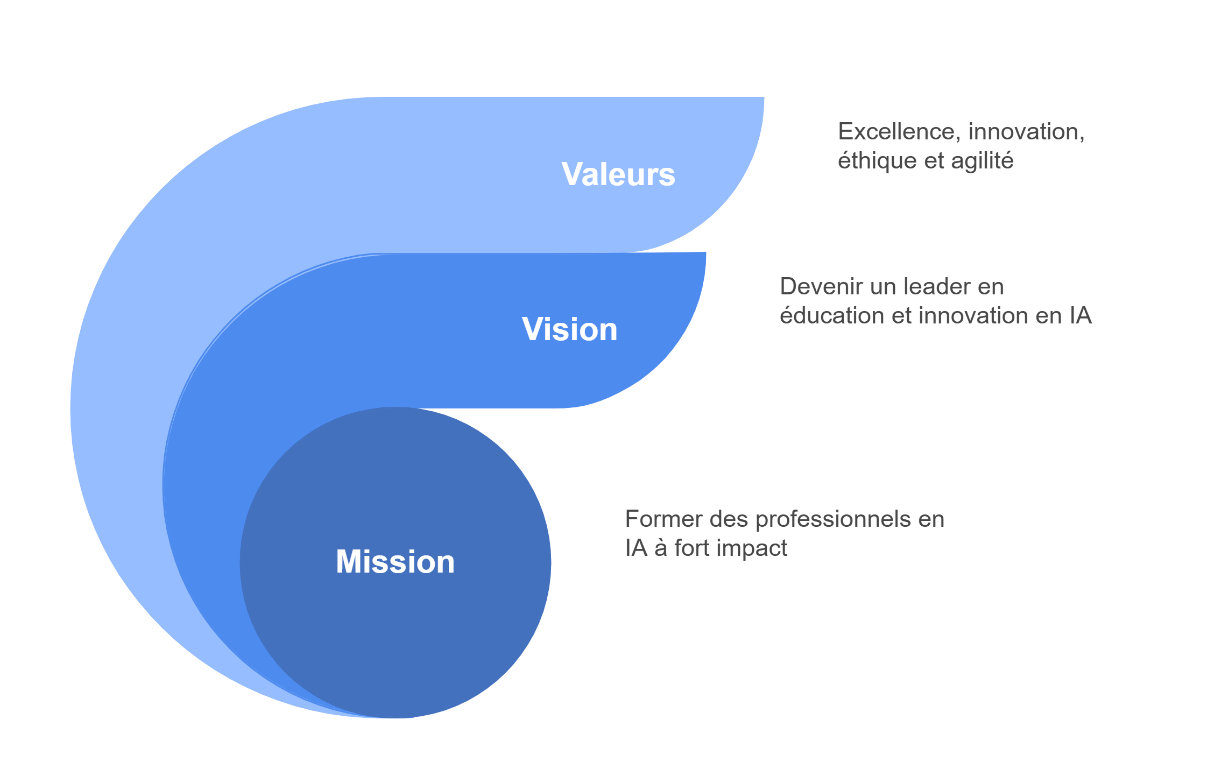
\includegraphics[width=0.8\textwidth]{images/mession.png}
  \caption{\textbf{Mission et vision de l'IAAI Academy}}
  \label{fig:mission}
\end{figure}

\begin{itemize}
  \item \textbf{Mission :} Former des professionnels capables de concevoir, déployer et piloter des solutions d'intelligence artificielle à fort impact, en s'appuyant sur une pédagogie innovante et des outils technologiques avancés.
  
  \item \textbf{Vision :} Devenir la référence au Maroc et en Afrique pour l'enseignement supérieur, l'innovation pédagogique et la recherche appliquée en IA, tout en contribuant à la transformation digitale du secteur éducatif.
  
  \item \textbf{Valeurs :}
  \begin{itemize}
    \item Excellence académique et exigence professionnelle
    \item Innovation pédagogique via l'intégration des technologies IA
    \item Éthique et esprit collaboratif
    \item Agilité et adaptabilité aux évolutions technologiques
  \end{itemize}
\end{itemize}

\section{Structure Organisationnelle et Gouvernance}

\begin{figure}[H]
  \centering
  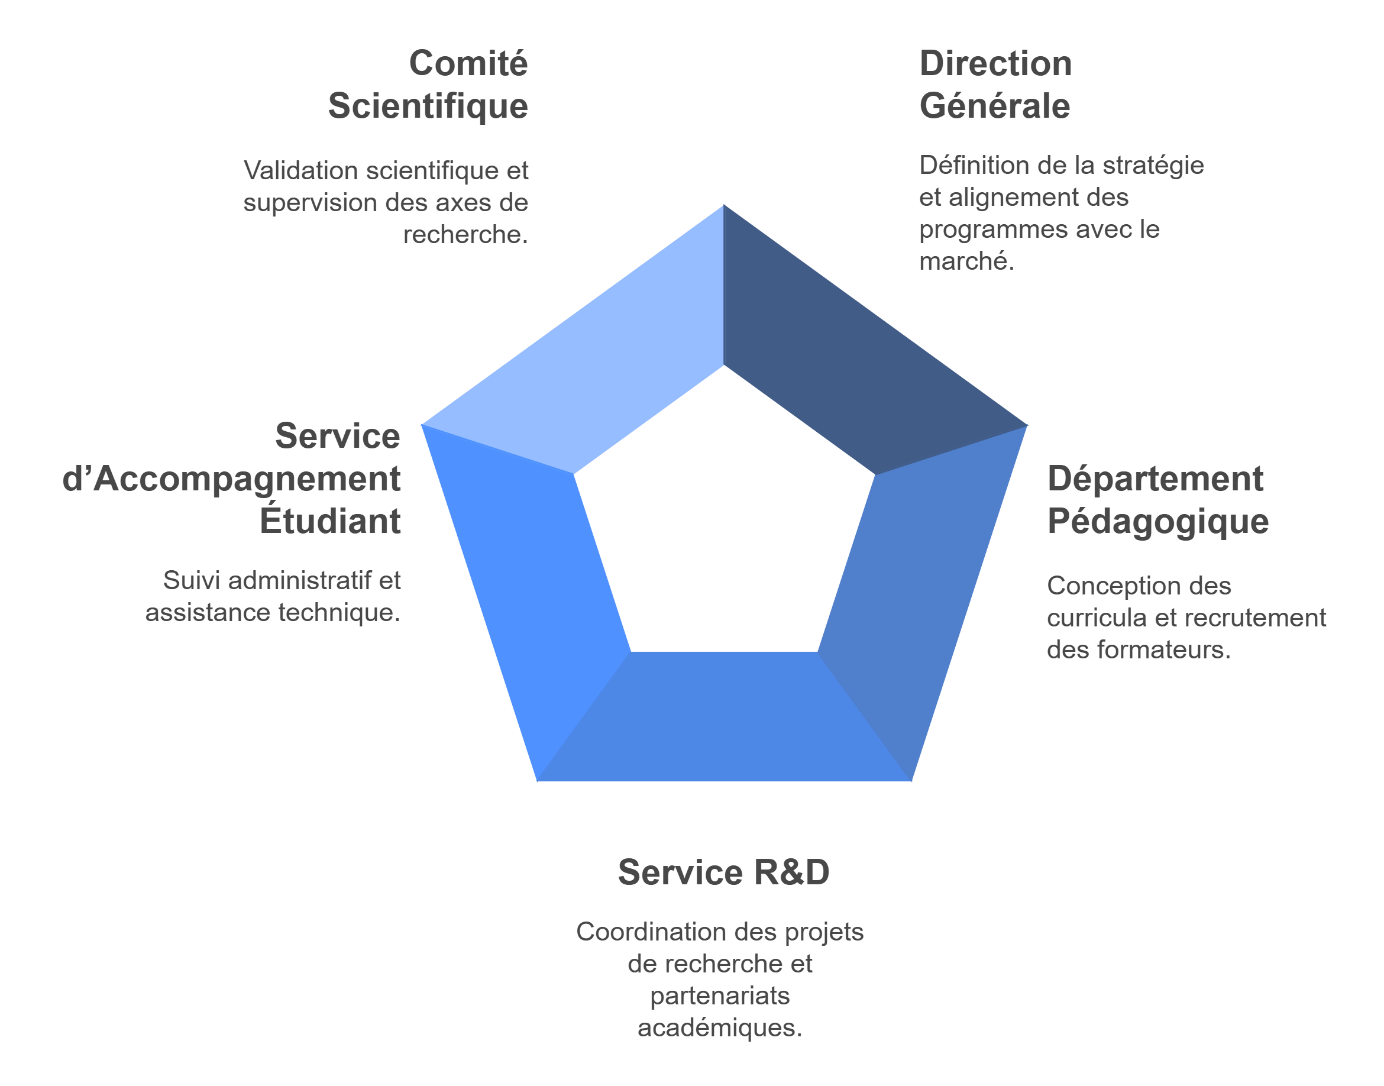
\includegraphics[width=0.9\textwidth]{images/Structure Organisationnelle et Gouvernance.png}
  \caption{\textbf{Organigramme et structure de gouvernance de l'IAAI Academy}}
  \label{fig:structure}
\end{figure}

L'IAAI Academy dispose d'une structure organisationnelle efficace, composée de plusieurs départements et unités qui travaillent en synergie pour atteindre les objectifs de l'institution. La gouvernance est assurée par un conseil d'administration et un comité exécutif qui définissent les orientations stratégiques et supervisent la mise en œuvre des projets.

\section{Offres de Formation et Domaines d'Intervention}

\begin{figure}[H]
  \centering
  \includegraphics[width=0.9\textwidth]{images/Offres de Formation et Domaines d'Intervention.png}
  \caption{\textbf{Panorama des formations et domaines d'expertise de l'IAAI Academy}}
  \label{fig:formations}
\end{figure}

\begin{itemize}
  \item \textbf{Formations professionnelles en IA et Data Science :}
  \begin{itemize}
    \item Modules intensifs (Python, Machine Learning, Deep Learning, NLP, vision par ordinateur)
    \item Certifications reconnues (IBM, Microsoft, Google, Coursera)
  \end{itemize}
  
  \item \textbf{Préparation aux concours post-bac :}
  \begin{itemize}
    \item Parcours pour médecine, pharmacie, ENSA/ENSAM, ENCG
    \item Formats présentiel, à distance ou hybride, avec examens blancs et coaching
  \end{itemize}
  
  \item \textbf{Soutien scolaire individualisé :}
  \begin{itemize}
    \item Cours sur mesure en mathématiques, physique-chimie, SVT et informatique
    \item Suivi des progrès, méthodes de travail et préparation aux examens
  \end{itemize}
  
  \item \textbf{Consulting et prestations IA :}
  \begin{itemize}
    \item Développement de chatbots, automatisation de processus et analyses prédictives
    \item Accompagnement à la transformation numérique
  \end{itemize}
  
  \item \textbf{Clubs technologiques et ateliers jeunesse :}
  \begin{itemize}
    \item Initiation à la programmation, robotique éducative et réalité augmentée
    \item Projets ludiques pour stimuler l'innovation dès le plus jeune âge
  \end{itemize}
\end{itemize}

\section{Pédagogie et Méthodes d'Apprentissage}

\begin{figure}[H]
  \centering
  \includegraphics[width=0.9\textwidth]{images/Pédagogie et Méthodes d'Apprentissage.png}
  \caption{\textbf{Approche pédagogique innovante de l'IAAI Academy}}
  \label{fig:pedagogie}
\end{figure}

L'IAAI Academy adopte une approche pédagogique innovante, intégrant les technologies d'intelligence artificielle pour personnaliser l'apprentissage et optimiser l'acquisition des compétences. Cette méthode combine enseignement théorique, pratique intensive et projets concrets, enrichis par des outils d'évaluation continue et d'adaptation du contenu au profil de chaque apprenant.

\section{Impact de mon Stage}

Ce stage m'a permis de :
\begin{itemize}
  \item M'immerger dans un environnement professionnel concret, en participant à des projets IA et pédagogiques
  \item Renforcer mes compétences en data science et technologies IA, ainsi qu'en développement Web (React) et mobile (React Native)
  \item Collaborer au sein d'une équipe pluridisciplinaire, développant ma capacité d'adaptation et de communication
  \item Adopter une posture critique et réflexive, afin de proposer des solutions innovantes et répondre aux enjeux réels du terrain
\end{itemize}

\section{Conclusion}

L'IAAI Academy a offert un cadre d'apprentissage et de recherche exemplaire, conjuguant ressources innovantes, démarche pédagogique assistée par IA et infrastructures technologiques avancées. Ce stage m'a non seulement permis de consolider mes compétences et de comprendre les enjeux de l'intégration de l'IA en contexte réel, mais il m'a également ouvert de nouvelles perspectives professionnelles et académiques dans le domaine de l'intelligence artificielle appliquée à l'éducation. 

% Chapter 2: Requirements and Specifications
\chapter*{Chapitre 2 : Cahier des Charges et Spécifications}
\addcontentsline{toc}{chapter}{Chapitre 2 : Cahier des Charges et Spécifications}
\thispagestyle{fancy}
\setcounter{section}{0}
\newpage

\section{Introduction}

Ce chapitre présente le cahier des charges et les spécifications du projet LearnExpert, une plateforme e-learning innovante développée au sein d'IAAI. Il détaille le contexte du projet, les objectifs visés, ainsi que l'analyse approfondie des besoins fonctionnels et non fonctionnels. Cette étape préliminaire est essentielle pour établir une vision claire du système à développer et pour guider efficacement les phases ultérieures de conception et d'implémentation.

Nous aborderons également les choix technologiques effectués pour répondre aux exigences du projet, en justifiant la sélection de chaque composant de la stack technique. Cette analyse des besoins et des technologies constitue le socle sur lequel reposera l'ensemble du développement de la plateforme LearnExpert.

\section{Présentation du Projet LearnExpert}

\subsection{Contexte et Problématique}
Le secteur de l'éducation en ligne connaît une croissance exponentielle, accélérée encore davantage par la pandémie mondiale qui a révélé les limites des plateformes d'apprentissage existantes. Dans ce contexte, plusieurs problématiques ont été identifiées :

\begin{itemize}
  \item Les plateformes actuelles proposent souvent un contenu générique et peu personnalisé
  \item Les méthodes d'apprentissage de la programmation restent trop théoriques, avec un manque d'interactivité
  \item Les apprenants font face à une fragmentation des ressources éducatives, nécessitant de naviguer entre différentes plateformes
  \item Les outils d'apprentissage ne s'adaptent pas au rythme et au niveau de chaque utilisateur
\end{itemize}

Face à ces défis, IAAI a décidé de développer LearnExpert, une plateforme innovante centrée sur l'apprentissage de la programmation et des technologies web.

\subsection{Objectifs du Projet}
Le projet LearnExpert vise à créer une plateforme d'apprentissage complète qui se distingue par :

\begin{itemize}
  \item Une approche centrée sur la pratique et l'interactivité pour l'apprentissage de la programmation
  \item Une personnalisation de l'expérience d'apprentissage grâce à l'IA
  \item Une intégration de contenus structurés et de haute qualité pour divers langages de programmation
  \item Une architecture évolutive permettant d'ajouter de nouvelles fonctionnalités et de nouveaux contenus
  \item Une expérience utilisateur fluide et engageante
\end{itemize}

L'objectif principal est de créer une plateforme qui accompagne efficacement les apprenants dans leur parcours d'acquisition de compétences techniques, qu'ils soient débutants ou développeurs expérimentés cherchant à se perfectionner.

\section{Analyse des Besoins}

\subsection{Besoins Fonctionnels}
Les fonctionnalités clés identifiées pour la plateforme LearnExpert sont :

\begin{itemize}
  \item \textbf{Gestion des utilisateurs et authentification}
    \begin{itemize}
      \item Inscription et connexion des utilisateurs
      \item Profils utilisateurs avec suivi de progression
      \item Système de rôles (apprenant, créateur de contenu, administrateur)
    \end{itemize}
  
  \item \textbf{Gestion des cours et contenus}
    \begin{itemize}
      \item Catalogue de cours organisé par catégories et niveaux
      \item Système de modules et de leçons structurés
      \item Support pour divers formats de contenu (texte, code, vidéo)
    \end{itemize}
  
  \item \textbf{Apprentissage interactif}
    \begin{itemize}
      \item Éditeur de code intégré avec exécution en temps réel
      \item Exercices pratiques et projets guidés
      \item Tests automatisés pour valider les compétences
    \end{itemize}
  
  \item \textbf{Analyse et suivi}
    \begin{itemize}
      \item Tableau de bord de progression pour les apprenants
      \item Statistiques d'utilisation pour les administrateurs
      \item Recommandations personnalisées basées sur les performances
    \end{itemize}
  
  \item \textbf{Interface d'administration}
    \begin{itemize}
      \item Gestion des utilisateurs et des permissions
      \item Création et édition de contenu éducatif
      \item Suivi des métriques de la plateforme
    \end{itemize}
\end{itemize}

\subsection{Besoins Non Fonctionnels}
Au-delà des fonctionnalités, plusieurs exigences non fonctionnelles ont été définies :

\begin{itemize}
  \item \textbf{Performance}
    \begin{itemize}
      \item Temps de chargement des pages inférieur à 2 secondes
      \item Capacité à supporter au moins 1000 utilisateurs simultanés
      \item Exécution rapide du code dans l'environnement intégré
    \end{itemize}
  
  \item \textbf{Sécurité}
    \begin{itemize}
      \item Protection des données personnelles des utilisateurs
      \item Isolation des environnements d'exécution de code
      \item Authentification robuste et gestion sécurisée des sessions
    \end{itemize}
  
  \item \textbf{Accessibilité et UX}
    \begin{itemize}
      \item Interface intuitive et responsive (mobile, tablette, desktop)
      \item Respect des standards d'accessibilité WCAG 2.1
      \item Support multilingue (initialement français et anglais)
    \end{itemize}
  
  \item \textbf{Évolutivité et maintenance}
    \begin{itemize}
      \item Architecture modulaire facilitant l'ajout de nouvelles fonctionnalités
      \item Documentation technique complète
      \item Tests automatisés couvrant les fonctionnalités critiques
    \end{itemize}
\end{itemize}

\section{Technologies et Outils}

\subsection{Stack Technologique}
Après analyse des besoins et des contraintes du projet, les technologies suivantes ont été sélectionnées :

\begin{itemize}
  \item \textbf{Frontend}
    \begin{itemize}
      \item Next.js (framework React) pour le développement d'une application web moderne
      \item TypeScript pour garantir la robustesse et la maintenabilité du code
      \item Tailwind CSS pour un design responsive et cohérent
      \item Monaco Editor pour l'implémentation de l'éditeur de code interactif
      \item Framer Motion pour les animations et transitions fluides
    \end{itemize}
  
  \item \textbf{Backend}
    \begin{itemize}
      \item Architecture microservices avec Node.js et Express
      \item NGINX comme API Gateway pour la gestion des requêtes
      \item Supabase pour l'authentification et les services de base de données
      \item MongoDB pour le stockage des contenus de cours et des données structurées
    \end{itemize}
  
  \item \textbf{Traitement des données}
    \begin{itemize}
      \item Python pour les scripts de scraping et de nettoyage de données
      \item APIs LLM (Large Language Models) pour le traitement intelligent des contenus
      \item JSON comme format principal pour le stockage et l'échange de données
    \end{itemize}
  
  \item \textbf{Déploiement et infrastructure}
    \begin{itemize}
      \item Vercel pour l'hébergement du frontend
      \item Docker pour la conteneurisation des services backend
      \item GitHub Actions pour l'intégration et le déploiement continus
    \end{itemize}
\end{itemize}

\subsection{Environnement de Développement}
L'environnement de développement a été soigneusement configuré pour maximiser la productivité, la collaboration et la qualité du code :

\begin{itemize}
  \item \textbf{Système d'exploitation :} 
  \begin{itemize}
    \item \textbf{Arch Linux :} Comme système principal, offrant une personnalisation poussée et des packages à jour
    \item \textbf{Hyprland :} Compositeur Wayland moderne et hautement configurable pour une interface fluide et efficace
    \item \textbf{Pacman :} Gestionnaire de paquets principal, complété par AUR (Arch User Repository) pour les applications tierces
  \end{itemize}
  
  \item \textbf{Éditeurs de code :} 
  \begin{itemize}
    \item \textbf{Neovim :} Éditeur principal avec une configuration personnalisée pour le développement web et React
    \item \textbf{Visual Studio Code :} IDE secondaire avec des extensions pour React, TypeScript, ESLint et Tailwind
  \end{itemize}
  
  \item \textbf{Terminal et multiplexeur :} 
  \begin{itemize}
    \item \textbf{Alacritty :} Émulateur de terminal GPU-accelerated pour des performances optimales
    \item \textbf{Tmux :} Pour la gestion de multiples sessions de travail et la persistance des environnements
    \item \textbf{Zsh :} Shell avec Oh-My-Zsh pour une productivité accrue et une expérience personnalisée
  \end{itemize}
  
  \item \textbf{Outils de développement :}
  \begin{itemize}
    \item \textbf{ESLint et Prettier :} Configuration personnalisée pour le linting et le formatage automatique du code
    \item \textbf{Chrome DevTools :} Pour le debugging et l'optimisation des performances frontend
    \item \textbf{React Developer Tools :} Extension pour l'analyse des composants React
    \item \textbf{Redux DevTools :} Pour le debugging de l'état global de l'application
  \end{itemize}
  
  \item \textbf{Gestion de versions et documentation :}
  \begin{itemize}
    \item \textbf{Git :} Avec une configuration avancée incluant des hooks personnalisés
    \item \textbf{GitHub :} Pour l'hébergement du code, la revue de code et la gestion des problèmes
    \item \textbf{GitHub Actions :} Pour l'intégration continue et le déploiement automatisé
    \item \textbf{Obsidian :} Pour la documentation, les notes de développement et la gestion des connaissances
  \end{itemize}
  
  \item \textbf{Outils de test et API :}
  \begin{itemize}
    \item \textbf{Postman :} Pour le test et la documentation des API
    \item \textbf{Jest et React Testing Library :} Pour les tests unitaires et d'intégration
    \item \textbf{Cypress :} Pour les tests end-to-end
  \end{itemize}
  
  \item \textbf{Design et UX :}
  \begin{itemize}
    \item \textbf{Figma :} Pour la conception et le prototypage de l'interface utilisateur
  \end{itemize}
  
  \item \textbf{Environnements virtualisés :}
  \begin{itemize}
    \item \textbf{Docker et Docker Compose :} Pour la conteneurisation des services et la cohérence des environnements
    \item \textbf{GNOME Boxes :} Pour la création de machines virtuelles isolées et le test dans différents environnements
    \item \textbf{nvm (Node Version Manager) :} Pour la gestion des versions de Node.js
    \item \textbf{pyenv :} Pour la gestion des environnements Python
  \end{itemize}
\end{itemize}

Cette stack technologique a été choisie pour sa modernité, sa flexibilité et sa capacité à répondre aux besoins spécifiques du projet, tout en garantissant des performances optimales et une bonne expérience utilisateur. 

\section{Planification et Gestion du Projet}

La planification du projet LearnExpert a été réalisée selon une approche méthodique, permettant de visualiser les différentes phases, les tâches associées, leurs durées et leurs interdépendances. Deux outils de visualisation complémentaires ont été utilisés pour représenter le planning du projet : le diagramme de Gantt et le diagramme PERT.

\subsection{Diagramme de Gantt}

Le diagramme de Gantt offre une représentation chronologique des tâches, permettant de visualiser :
\begin{itemize}[leftmargin=*,noitemsep,topsep=0pt]
  \item La durée de chaque tâche
  \item Les dates de début et de fin
  \item Le chevauchement entre les différentes tâches
  \item La répartition des tâches par phase du projet
\end{itemize}

\begin{figure}[htb]
  \centering
  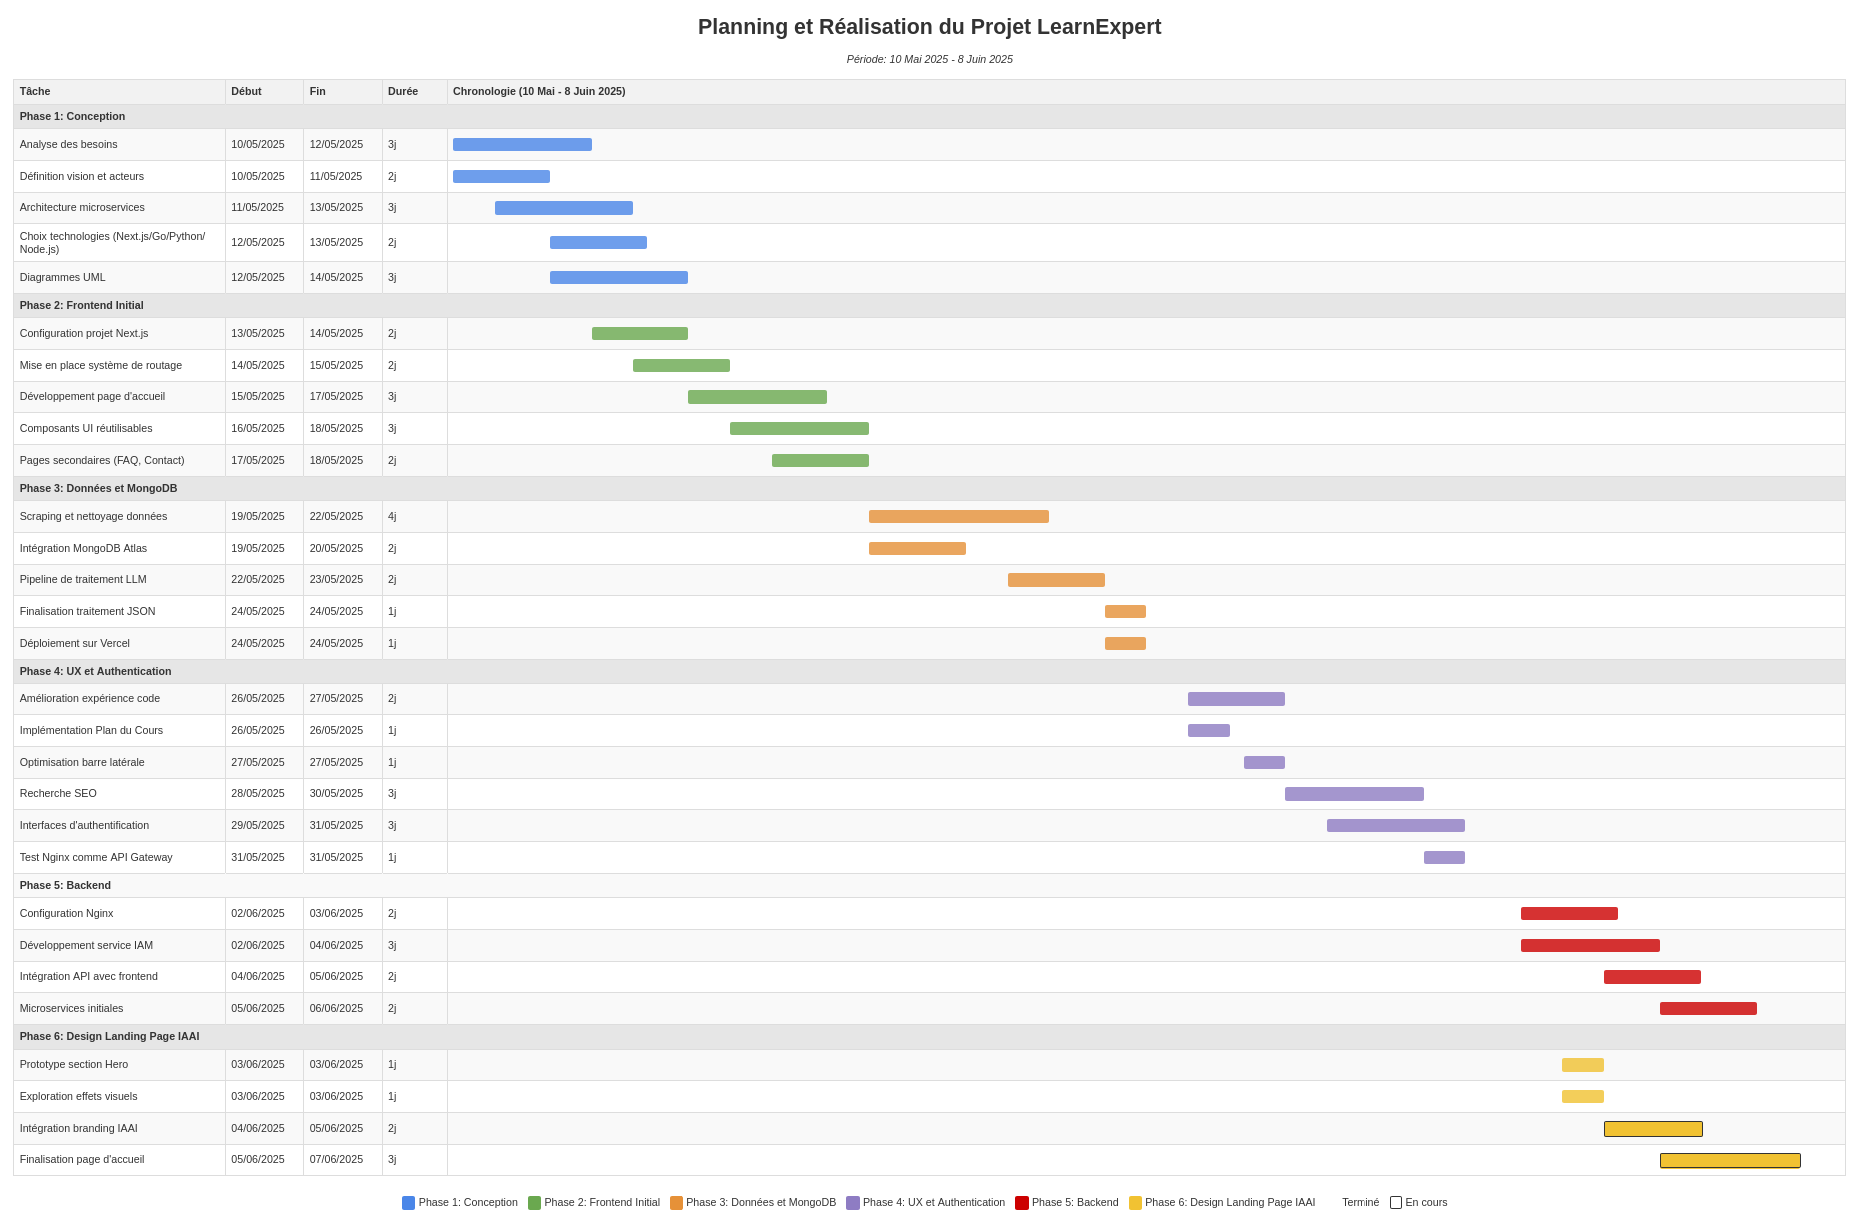
\includegraphics[width=0.9\textwidth,keepaspectratio]{images/gestion_projet/gantt_diagram.png}
  \caption{\textbf{Diagramme de Gantt} montrant la planification et la progression du projet.}
  \label{fig:gantt_diagram}
\end{figure}

Ce diagramme permet d'identifier clairement la durée totale du projet (du 10 mai au 8 juin 2025) ainsi que les périodes d'activité intense où plusieurs tâches se déroulent en parallèle. On peut notamment constater que les phases 1 à 3 (Conception, Frontend initial, Données et MongoDB) se déroulent principalement durant la première moitié du projet, tandis que les phases 4 à 6 (UX et Authentification, Backend, Design Landing Page) occupent la seconde moitié.

\subsection{Diagramme PERT}
Le diagramme PERT (Program Evaluation and Review Technique) complète le diagramme de Gantt en illustrant les dépendances entre les tâches et le chemin critique du projet.

\begin{figure}[htb]
  \centering
  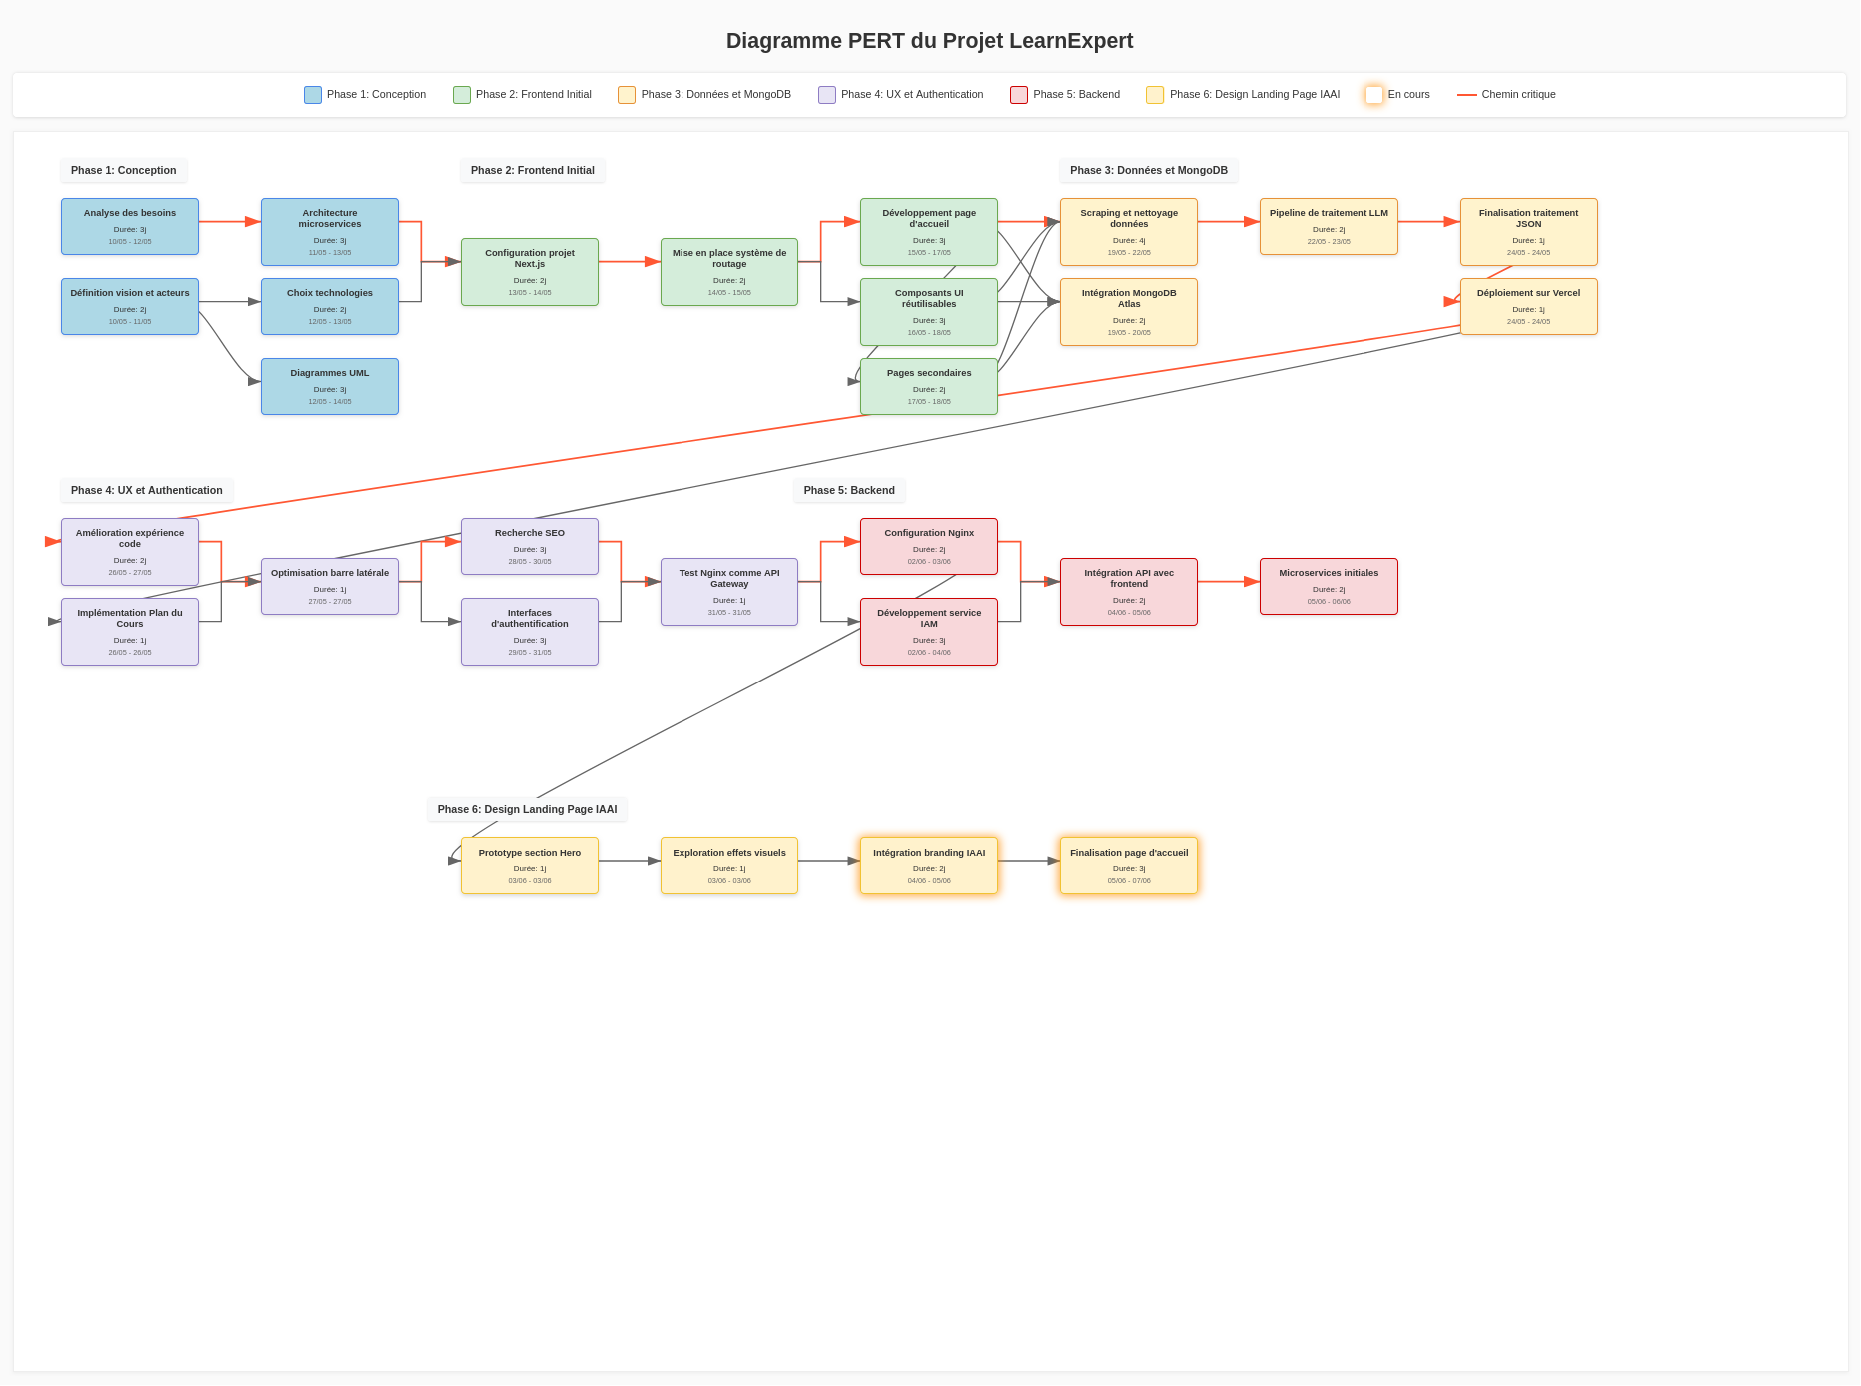
\includegraphics[width=0.9\textwidth,keepaspectratio]{images/gestion_projet/pert_diagram.png}
  \caption{\textbf{Diagramme PERT} montrant les relations et dépendances entre les tâches du projet.}
  \label{fig:pert_diagram}
\end{figure}

L'analyse du diagramme PERT permet de dégager plusieurs observations importantes :

\begin{itemize}[leftmargin=*,noitemsep,topsep=0pt]
  \item \textbf{Organisation modulaire} : Les tâches sont regroupées en six phases distinctes, chacune avec ses propres objectifs et livrables.
  
  \item \textbf{Dépendances inter-phases} : Certaines tâches de phases ultérieures dépendent de l'achèvement de tâches de phases antérieures, ce qui souligne l'importance de respecter les jalons intermédiaires.
  
  \item \textbf{Chemin critique} : Représenté en rouge, le chemin critique identifie les tâches dont tout retard impacterait directement la date de fin du projet. Il traverse notamment les phases de conception, de développement frontend, de pages secondaires, et s'étend jusqu'aux services backend.
  
  \item \textbf{Parallélisation des tâches} : Plusieurs activités peuvent être menées en parallèle, comme le développement des composants UI et la mise en place du système de routage, optimisant ainsi l'utilisation des ressources.
\end{itemize}

\subsection{Avantages de la Planification Visuelle}

L'utilisation combinée des diagrammes de Gantt et PERT présente plusieurs avantages significatifs pour la gestion du projet :

\begin{itemize}[leftmargin=*,noitemsep,topsep=0pt]
  \item \textbf{Communication claire} : Facilite la compréhension du planning par toutes les parties prenantes, techniques et non techniques.
  
  \item \textbf{Identification des risques} : Permet de repérer les zones de tension potentielles dans le planning, notamment les tâches sur le chemin critique.
  
  \item \textbf{Suivi de l'avancement} : Offre un référentiel visuel pour mesurer la progression réelle par rapport au planning initial.
  
  \item \textbf{Allocation des ressources} : Aide à l'optimisation de l'attribution des ressources humaines et techniques sur les différentes tâches.
  
  \item \textbf{Anticipation des dépendances} : Met en évidence les relations entre les tâches, permettant de préparer à l'avance les transitions entre phases.
\end{itemize}

La planification détaillée réalisée pour le projet LearnExpert constitue un élément essentiel pour assurer une exécution maîtrisée et respecter les délais fixés. Elle servira de référence tout au long du développement pour suivre l'avancement et ajuster les priorités si nécessaire.

\section{Conclusion}

Le cahier des charges présenté dans ce chapitre définit les fondements du projet LearnExpert, établissant clairement le contexte, les objectifs et les spécifications techniques nécessaires à sa réalisation. Face aux défis identifiés dans le secteur de l'éducation en ligne, la plateforme ambitionne d'apporter une solution innovante centrée sur l'apprentissage interactif de la programmation et des technologies web.

L'analyse approfondie des besoins fonctionnels et non fonctionnels a permis d'établir un cadre précis pour le développement, avec un accent particulier sur l'expérience utilisateur, la performance et la sécurité. La structure modulaire envisagée pour la plateforme favorisera son évolutivité et sa maintenance sur le long terme.

Le choix des technologies, notamment Next.js pour le frontend, une architecture microservices pour le backend, et l'utilisation de modèles de langage large pour le traitement des données, témoigne d'une approche moderne et adaptée aux exigences du projet. Cette sélection technique offre un équilibre optimal entre performance, flexibilité et facilité de développement, posant ainsi les bases solides pour la phase de conception et d'implémentation qui suivra.

Une planification rigoureuse du projet a été établie à l'aide des diagrammes de Gantt et PERT, permettant une visualisation claire des phases, des tâches et de leurs interdépendances. Cette organisation méthodique constitue un atout majeur pour le bon déroulement du projet dans les délais impartis.

Cette phase préparatoire constitue une étape cruciale dans le cycle de vie du projet, fournissant une vision claire et des directives précises pour guider efficacement les phases ultérieures de développement. 

% Chapter 3: Platform Design and Architecture
\chapter{Chapitre 3 : Conception et Modélisation}
\thispagestyle{fancy}
\newpage

\section{Introduction}
La première phase du projet a été consacrée à la conception initiale, à la définition de l'architecture backend et des bases de données, ainsi qu'à la création des premiers diagrammes UML.

\section{Méthodologie Adoptée}
La méthodologie adoptée pour la conception du système s'est basée sur une approche structurée et itérative.

\subsection{Modèle en cascade}
Pour la phase de conception, nous avons adopté une approche en cascade adaptée, permettant de définir clairement les étapes successives tout en maintenant la possibilité de réviser les décisions précédentes au besoin.

\subsection{Langage UML}
Le langage UML (Unified Modeling Language) a été utilisé comme standard pour représenter graphiquement l'architecture et les interactions du système. Ce choix permet une communication claire et non ambiguë entre toutes les parties prenantes du projet.

\section{Conception}

\subsection{Identification des acteurs}
Les principaux types d'utilisateurs identifiés pour la plateforme sont :
\begin{itemize}
  \item \textbf{Apprenant Individuel :} S'inscrit, s'abonne, apprend, demande des consultations
  \item \textbf{Employé d'Entreprise :} Apprend via l'abonnement de l'entreprise, demande des consultations
  \item \textbf{Administrateur/Manager d'Entreprise :} Gère le compte de l'entreprise, les employés, les abonnements, attribue les cours, consulte les analyses
  \item \textbf{Créateur de Cours :} Conçoit et élabore le contenu des cours (modules, leçons, quiz)
  \item \textbf{Consultant/Fournisseur de Prestations :} Gère sa disponibilité, anime les sessions via la plateforme de réunion
  \item \textbf{Agent de Support Plateforme :} Assiste les utilisateurs pour les problèmes liés à la plateforme et les questions-réponses
  \item \textbf{Administrateur de la Plateforme :} Supervise l'ensemble de la plateforme, les utilisateurs, le contenu, les paramètres
\end{itemize}

\subsection{Identification des messages}
La plateforme e-learning conçue repose sur les fonctionnalités essentielles suivantes :
\begin{itemize}
    \item \textbf{E-Learning :}
    \begin{itemize}
        \item Catalogue de cours (filtrable, consultable)
        \item Modules, Leçons (vidéo, basées sur des images)
        \item Quiz et Évaluations
        \item Suivi de la Progression
        \item Certificats de Réussite
        \item Support Multilingue (EN/FR)
        \item Paramètres Utilisateur et Entreprise
    \end{itemize}
    \item \textbf{Consultation et Prestation :}
    \begin{itemize}
        \item Navigation des services
        \item Profils des consultants et disponibilité
        \item Système de réservation/demande
        \item Intégration API avec la plateforme de réunion personnalisée
        \item Facturation des sessions
    \end{itemize}
    \item \textbf{Monétisation :}
    \begin{itemize}
        \item Abonnements pour utilisateurs individuels (accès illimité)
        \item Abonnements pour entreprises (par utilisateur)
        \item Réductions et Démos
    \end{itemize}
\end{itemize}

\subsection{Les diagrammes de cas d'utilisation}
Les diagrammes de cas d'utilisation ont permis de représenter visuellement les interactions entre les acteurs et le système.

\begin{figure}[h!]
  \centering
  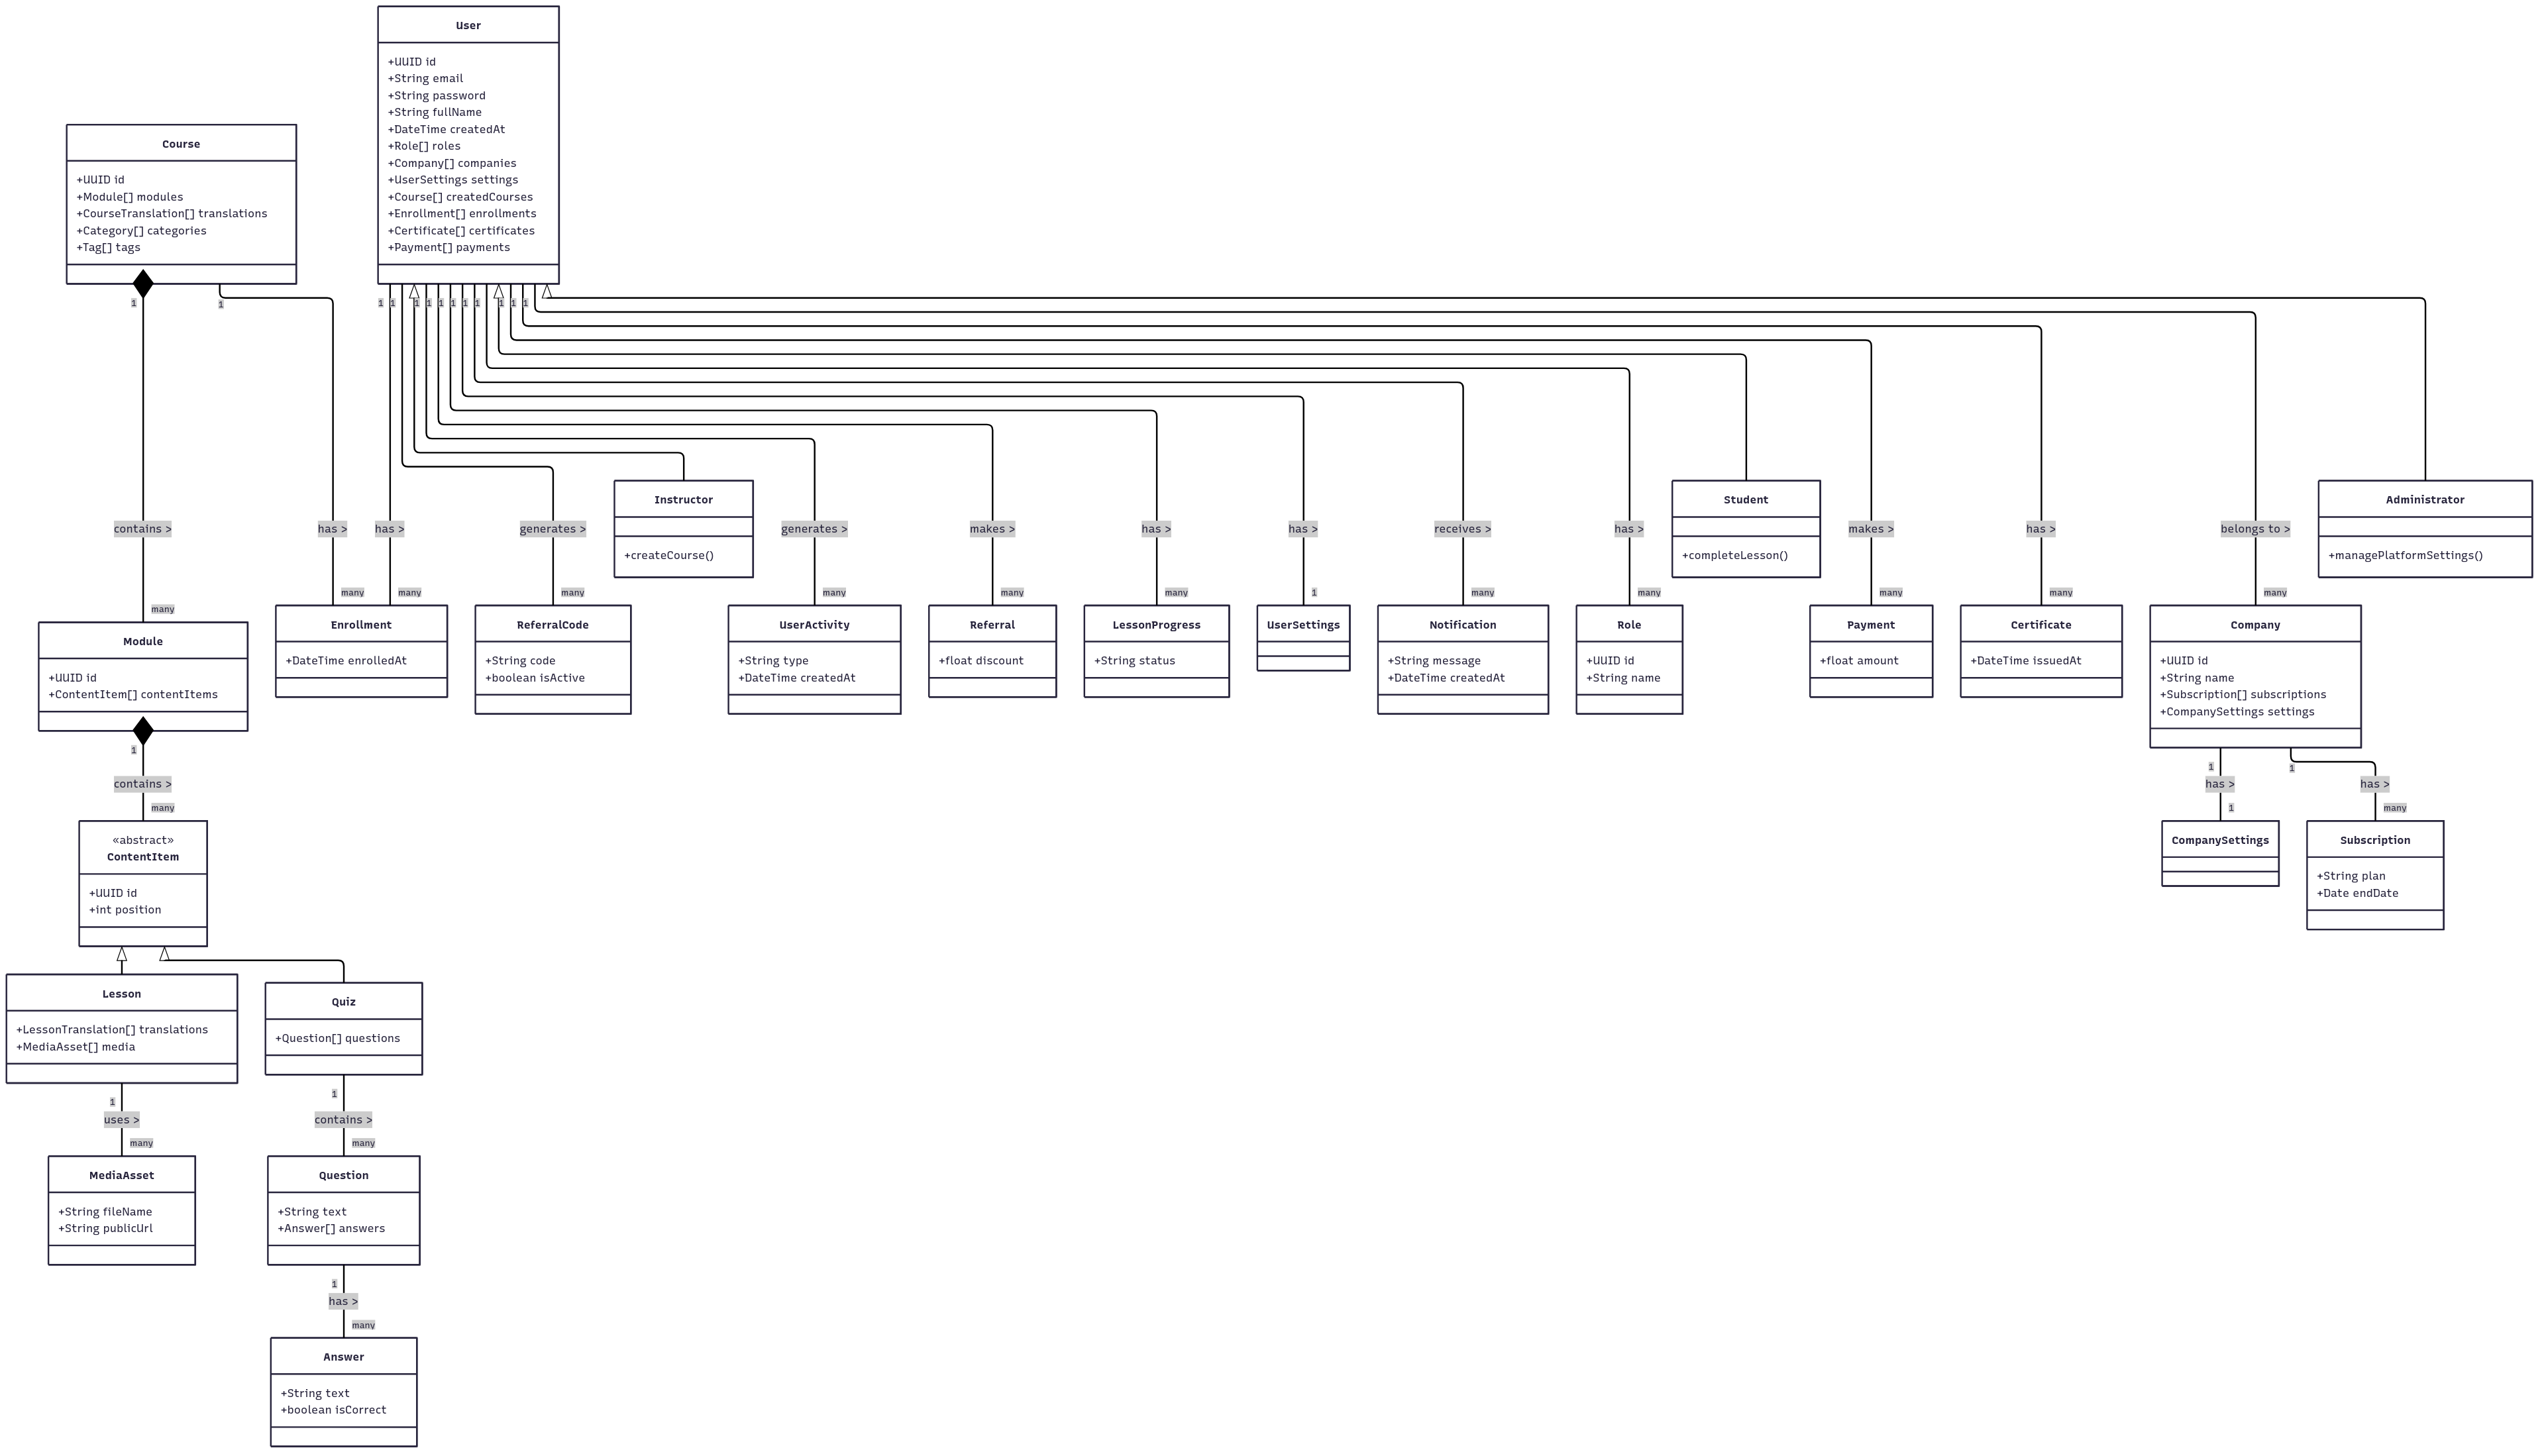
\includegraphics[width=0.9\textwidth,keepaspectratio]{class_diagrame.png}
  \caption{\textbf{Diagramme de cas d'utilisation} montrant les principales fonctionnalités accessibles par les acteurs.}
  \label{fig:usecase_diagram}
\end{figure}

\subsection{Les diagrammes de séquence}
Les diagrammes de séquence ont permis d'illustrer les interactions temporelles entre les différents composants du système pour des scénarios clés.

Pour illustrer le fonctionnement de l'architecture, voici un exemple de flux de communication entre les services pour un scénario d'inscription et d'abonnement :
\begin{enumerate}
  \item \textbf{Client (Next.js)} $\rightarrow$ \textbf{Passerelle API (Nginx)} $\rightarrow$ \textbf{Service IAM} (Création de l'utilisateur)
  \item \textbf{Service IAM} $\rightarrow$ \textbf{Kafka} (Publie `UserRegisteredEvent`)
  \item \textbf{Service de Notification} (Consomme l'événement) $\rightarrow$ Envoie un Email de Bienvenue
  \item \textbf{Client} $\rightarrow$ \textbf{Passerelle API} $\rightarrow$ \textbf{Service de Facturation} (Demande d'abonnement)
  \item \textbf{Service de Facturation} $\rightarrow$ Passerelle de Paiement et Mise à jour de la BD interne
  \item \textbf{Service de Facturation} $\rightarrow$ \textbf{Kafka} (Publie `SubscriptionActivatedEvent`)
  \item \textbf{Service IAM} (Consomme, met à jour le statut utilisateur) \& \textbf{Service de Notification} (Consomme, envoie une confirmation)
\end{enumerate}

\begin{figure}[h!]
  \centering
  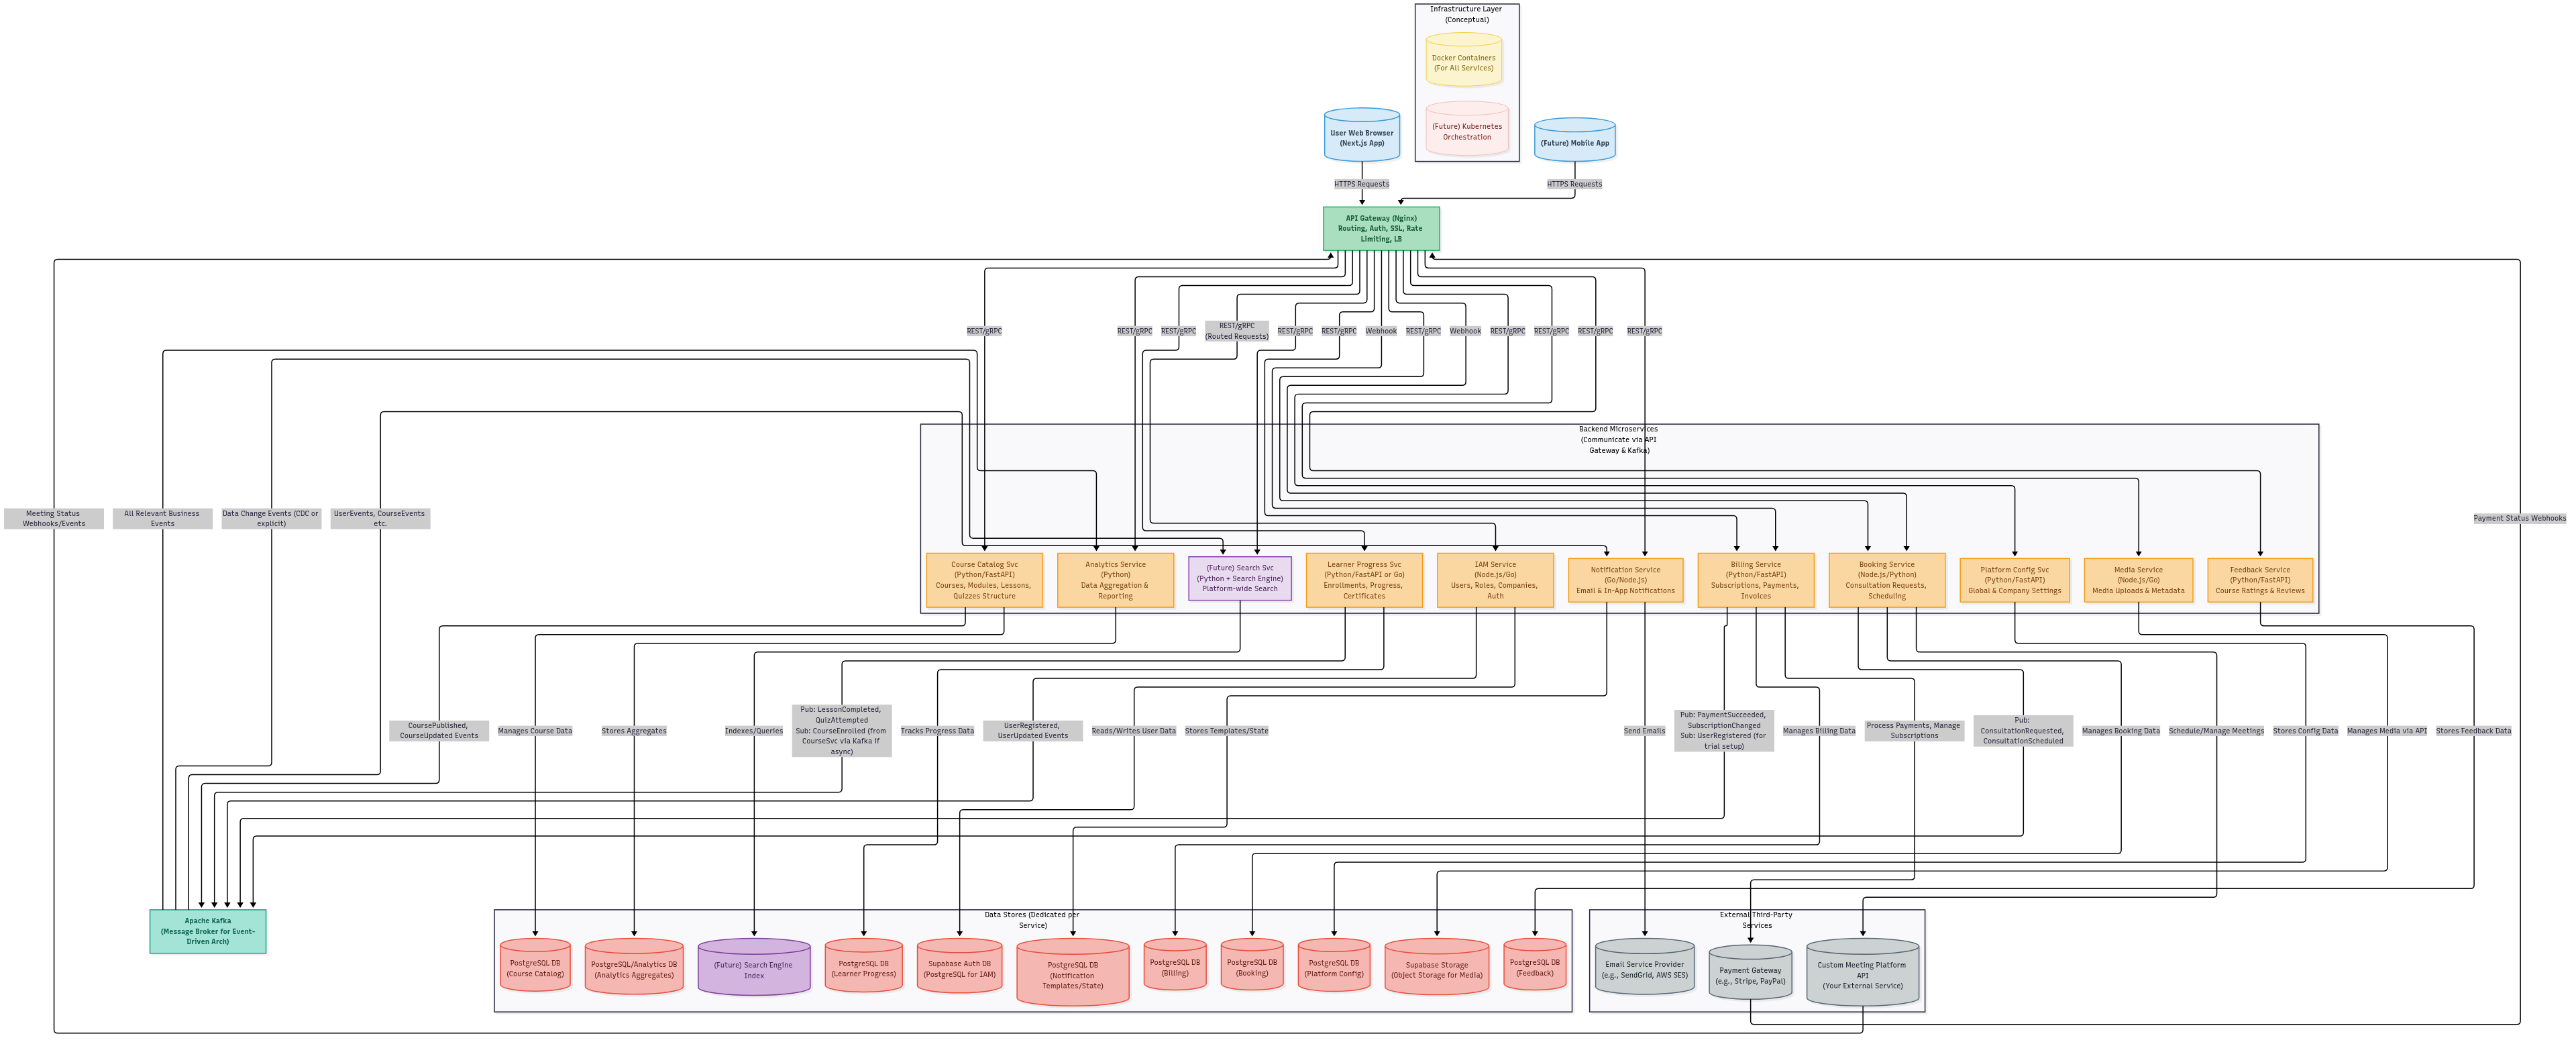
\includegraphics[width=0.9\textwidth,keepaspectratio]{archetecture_diagrame.png}
  \caption{\textbf{Diagramme de séquence} illustrant le processus d'inscription et d'abonnement.}
  \label{fig:sequence_diagram}
\end{figure}

\subsection{Le diagramme de classes}
Le diagramme de classes a été élaboré pour représenter les principales entités du système et leurs relations.

\begin{figure}[h!]
  \centering
  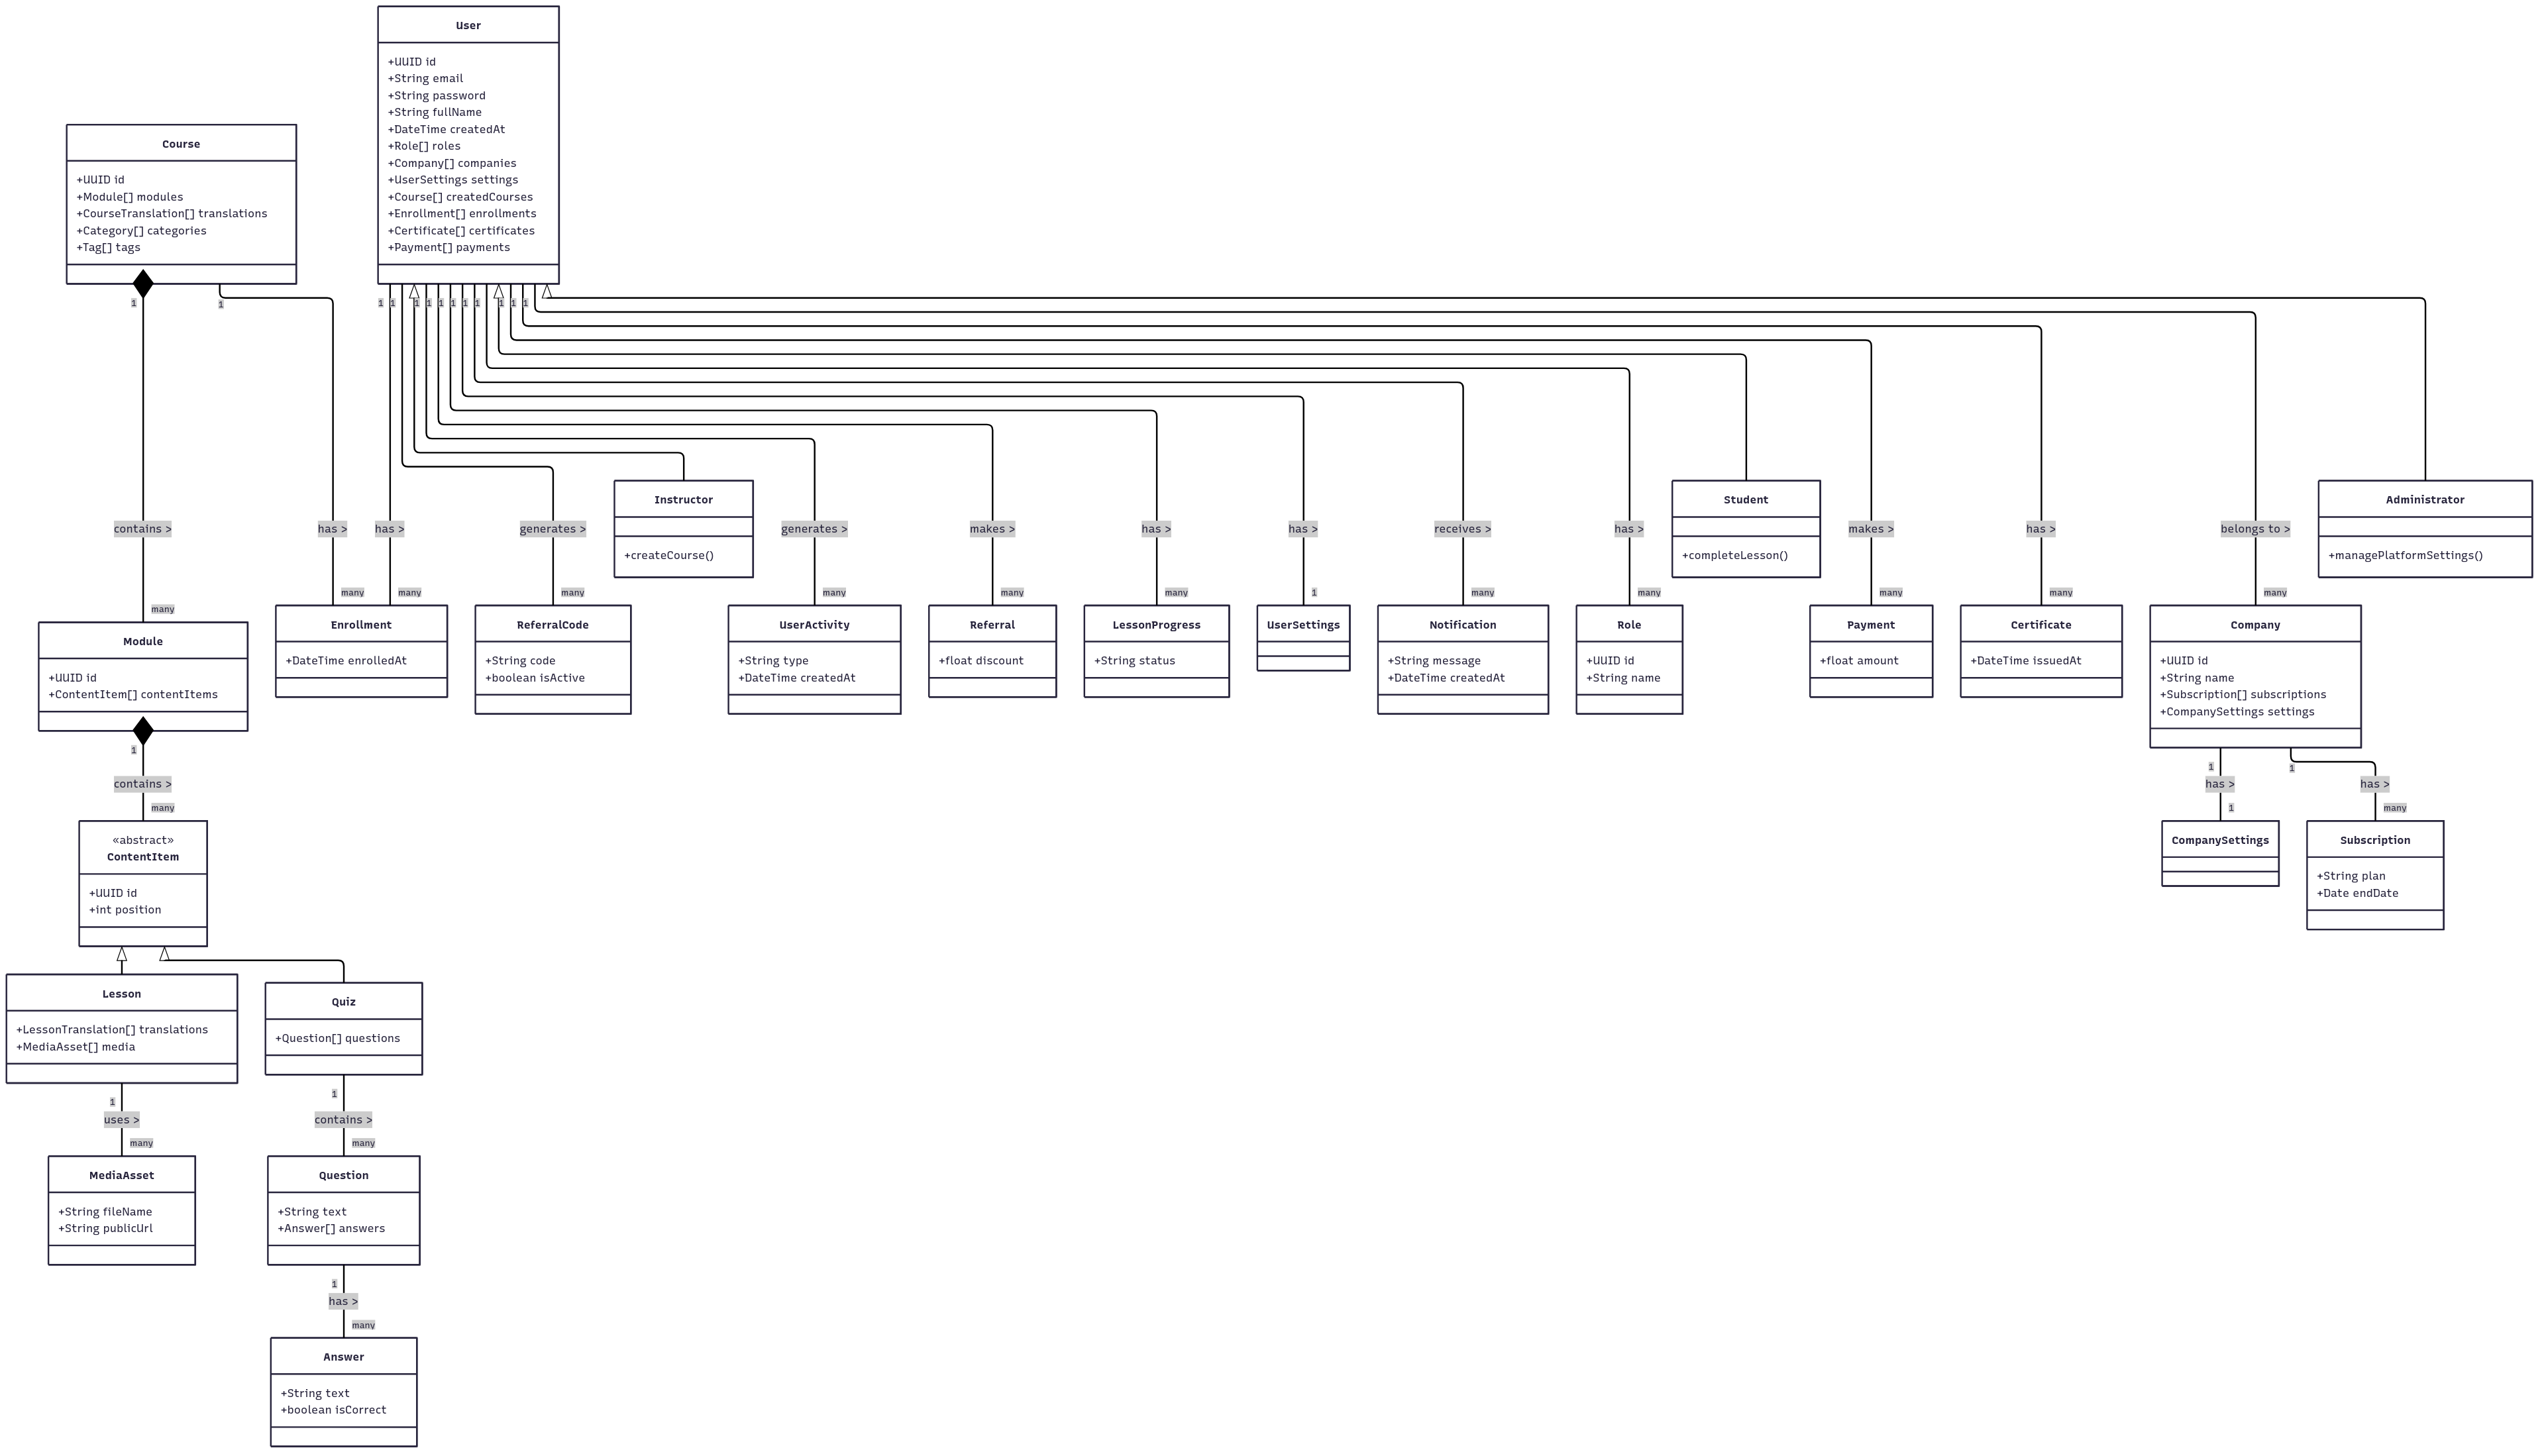
\includegraphics[width=0.9\textwidth,keepaspectratio]{class_diagrame.png}
  \caption{\textbf{Diagramme de classes} de la plateforme e-learning montrant les principales entités et leurs relations.}
  \label{fig:class_diagram}
\end{figure}

Ce diagramme illustre les relations entre les différentes entités du système, comme les utilisateurs, les cours, les modules, les leçons, les abonnements et les services de consultation. Les cardinalités et les types de relations (composition, agrégation, héritage) ont été définies pour refléter précisément la structure du modèle de données.

\section{Architecture Adoptée}

L'architecture envisagée pour la plateforme repose sur une approche de microservices, justifiée par plusieurs avantages clés :
\begin{itemize}
  \item \textbf{Scalabilité :} Mise à l'échelle indépendante des services individuels selon les besoins
  \item \textbf{Maintenabilité :} Possibilité de modifier des parties spécifiques sans impacter l'ensemble du système
  \item \textbf{Résilience :} Limitation de l'impact des défaillances à des services spécifiques
  \item \textbf{Autonomie des Équipes :} Développement, tests et déploiement indépendants par différentes équipes
  \item \textbf{Flexibilité Technologique :} Utilisation des technologies les plus adaptées pour chaque service
\end{itemize}

\subsection{Pile Technologique}
La pile technologique définie pour le développement comprend :
\begin{itemize}
  \item \textbf{Frontend :} Next.js (React)
  \item \textbf{Microservices Backend :}
    \begin{itemize}
      \item Go (pour les services critiques en performance et concurrents comme les Notifications, le backend de la plateforme de réunion)
      \item Python avec FastAPI (pour les services gourmands en données, développement rapide d'API, par exemple, Catalogue de Cours, Facturation)
      \item Node.js avec Express (TypeScript) (pour les opérations I/O intensives, interaction Supabase, par exemple, IAM, Gestion des Médias)
    \end{itemize}
  \item \textbf{Bases de Données :}
    \begin{itemize}
      \item PostgreSQL (stockage relationnel principal pour la plupart des services)
      \item Supabase (pour l'Authentification, le Stockage, et son Postgres géré pour des services spécifiques)
    \end{itemize}
  \item \textbf{Passerelle API :} Nginx (en tant que reverse proxy et passerelle)
  \item \textbf{Broker de Messages :} Apache Kafka (pour une gestion d'événements asynchrones robuste et scalable)
  \item \textbf{Conteneurisation et Orchestration :} Docker (Kubernetes serait une étape logique suivante pour l'orchestration)
\end{itemize}

\subsection{Modèles de Données des Services}
Dans le cadre de cette première phase, des modèles de données préliminaires ont été conçus pour chacun des services identifiés. Voici quelques exemples des structures de données principales :

\newpage
\subsubsection{Service IAM (Identity and Access Management)}
\begin{figure}[h!]
  \centering
  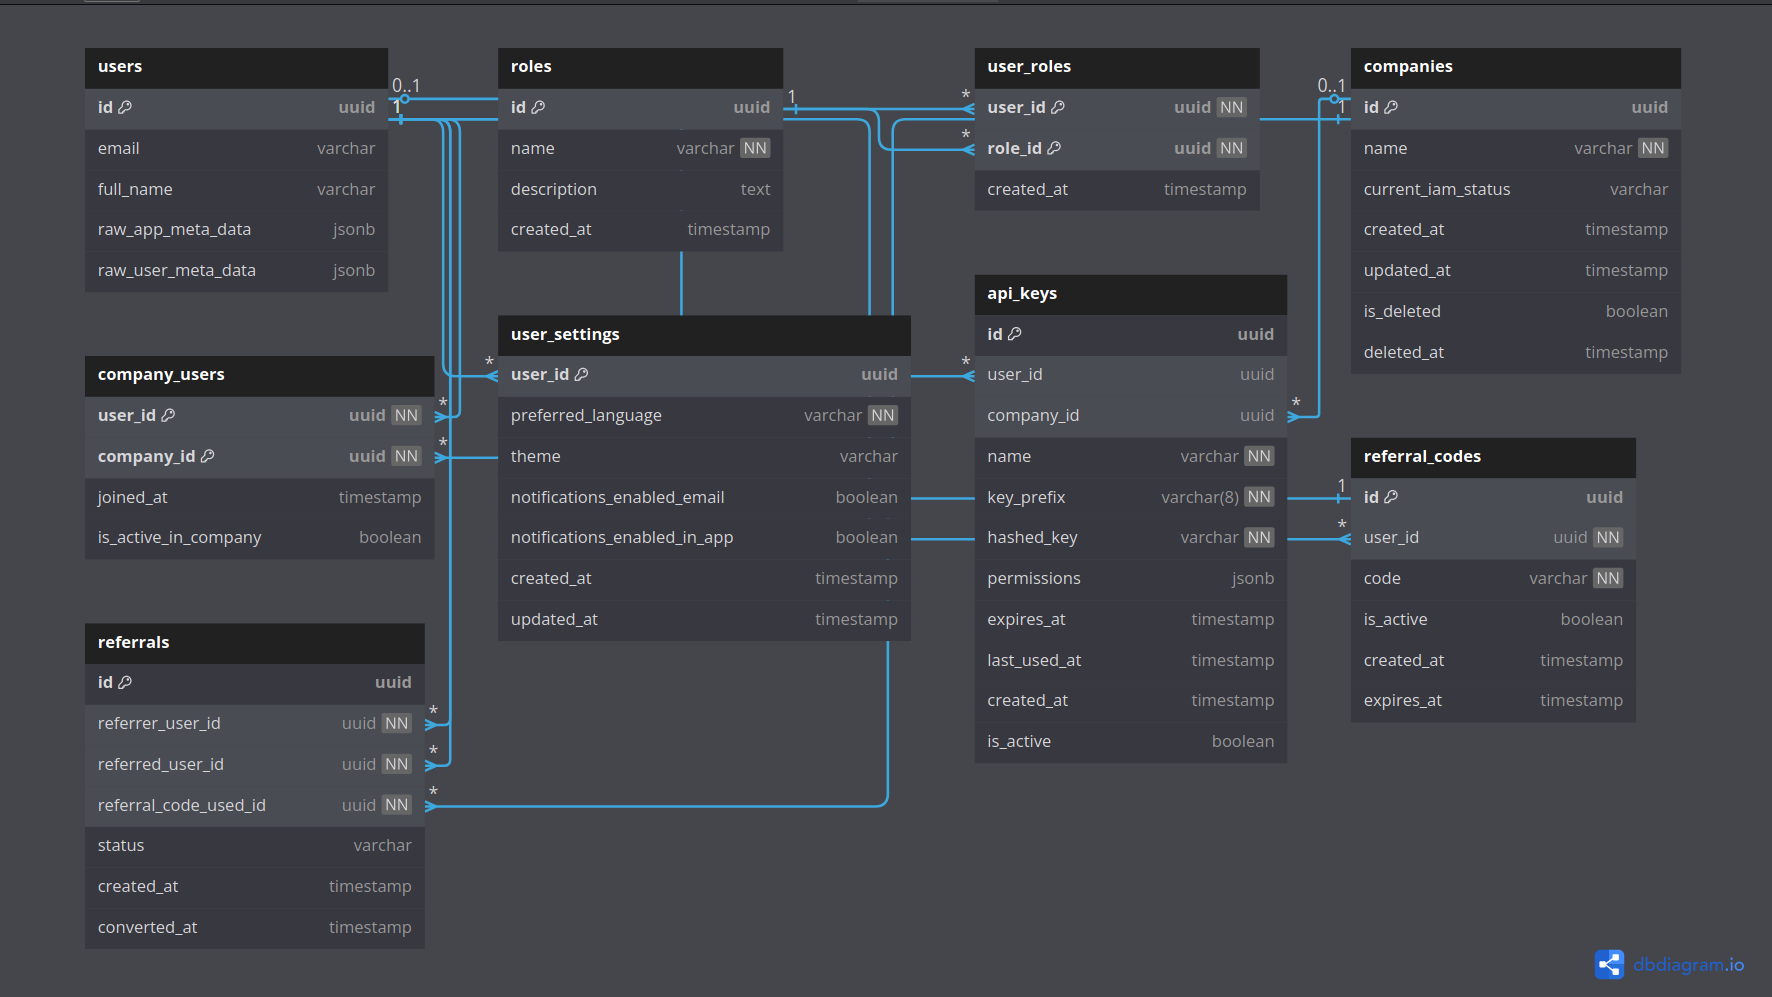
\includegraphics[width=0.8\textwidth,keepaspectratio]{services_db_screanshots/Screenshot 2025-06-06 at 15-08-36 IAM_Service.pdf.png}
  \caption{\textbf{Modèle de données du service IAM} pour la gestion des utilisateurs et des accès.}
  \label{fig:iam_service}
\end{figure}
\vspace{-10pt}
\small
\paragraph{Points clés du modèle IAM :}
\begin{itemize}[leftmargin=*,noitemsep,topsep=0pt]
  \item \textbf{Gestion centralisée des utilisateurs} avec tables dédiées aux utilisateurs, rôles et permissions
  \item \textbf{Support multi-tenant} via la table des entreprises (companies)
  \item \textbf{Système de référence} permettant le suivi des recommandations et affiliations
  \item \textbf{Paramètres utilisateurs} stockés de manière structurée pour personnaliser l'expérience
  \item \textbf{Jetons d'authentification} permettant une gestion sécurisée des sessions
\end{itemize}
\normalsize
\newpage

\subsubsection{Service de Contenu}
\begin{figure}[h!]
  \centering
  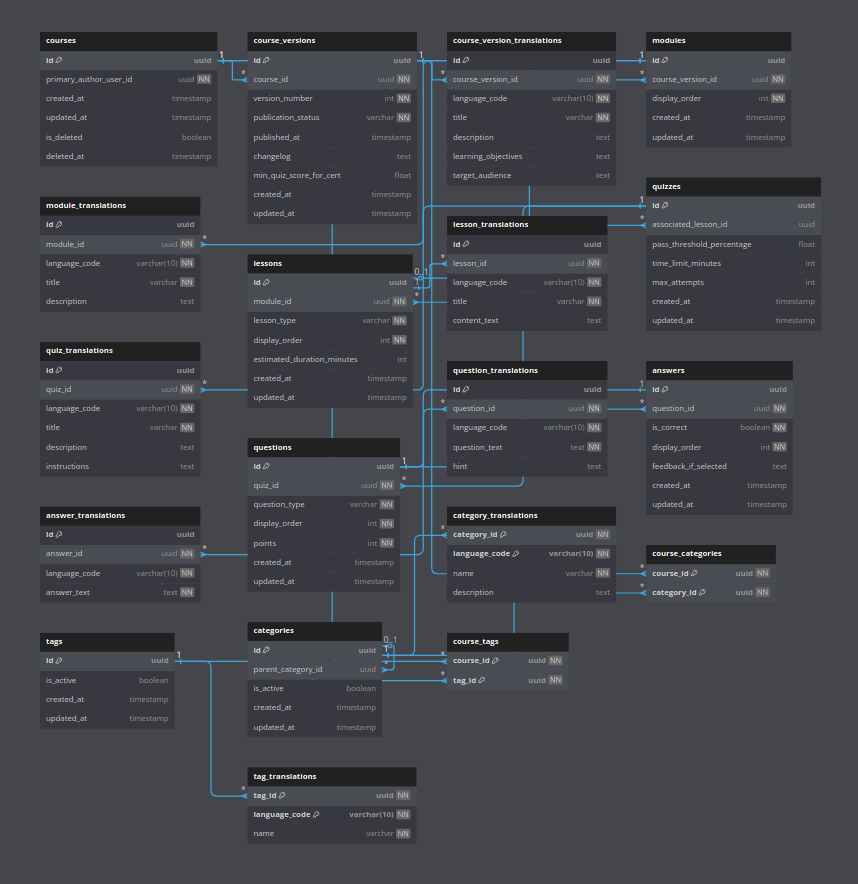
\includegraphics[width=0.8\textwidth,keepaspectratio]{services_db_screanshots/Screenshot 2025-06-06 at 15-07-51 Content_Service.pdf.png}
  \caption{\textbf{Modèle de données du service de contenu} pour la gestion des cours et du matériel pédagogique.}
  \label{fig:content_service}
\end{figure}
\vspace{-10pt}
\small
\paragraph{Points clés du service de Contenu :}
\begin{itemize}[leftmargin=*,noitemsep,topsep=0pt]
  \item \textbf{Structure hiérarchique} des cours, modules et leçons
  \item \textbf{Support multimédia} avec gestion des vidéos, documents et quizz
  \item \textbf{Métadonnées riches} pour faciliter la recherche et la catégorisation
  \item \textbf{Gestion des versions} permettant la mise à jour du contenu sans perte d'historique
  \item \textbf{Support multilingue} pour internationaliser le contenu pédagogique
\end{itemize}
\normalsize
\newpage

\subsubsection{Service de Facturation et d'Abonnement}
\begin{figure}[h!]
  \centering
  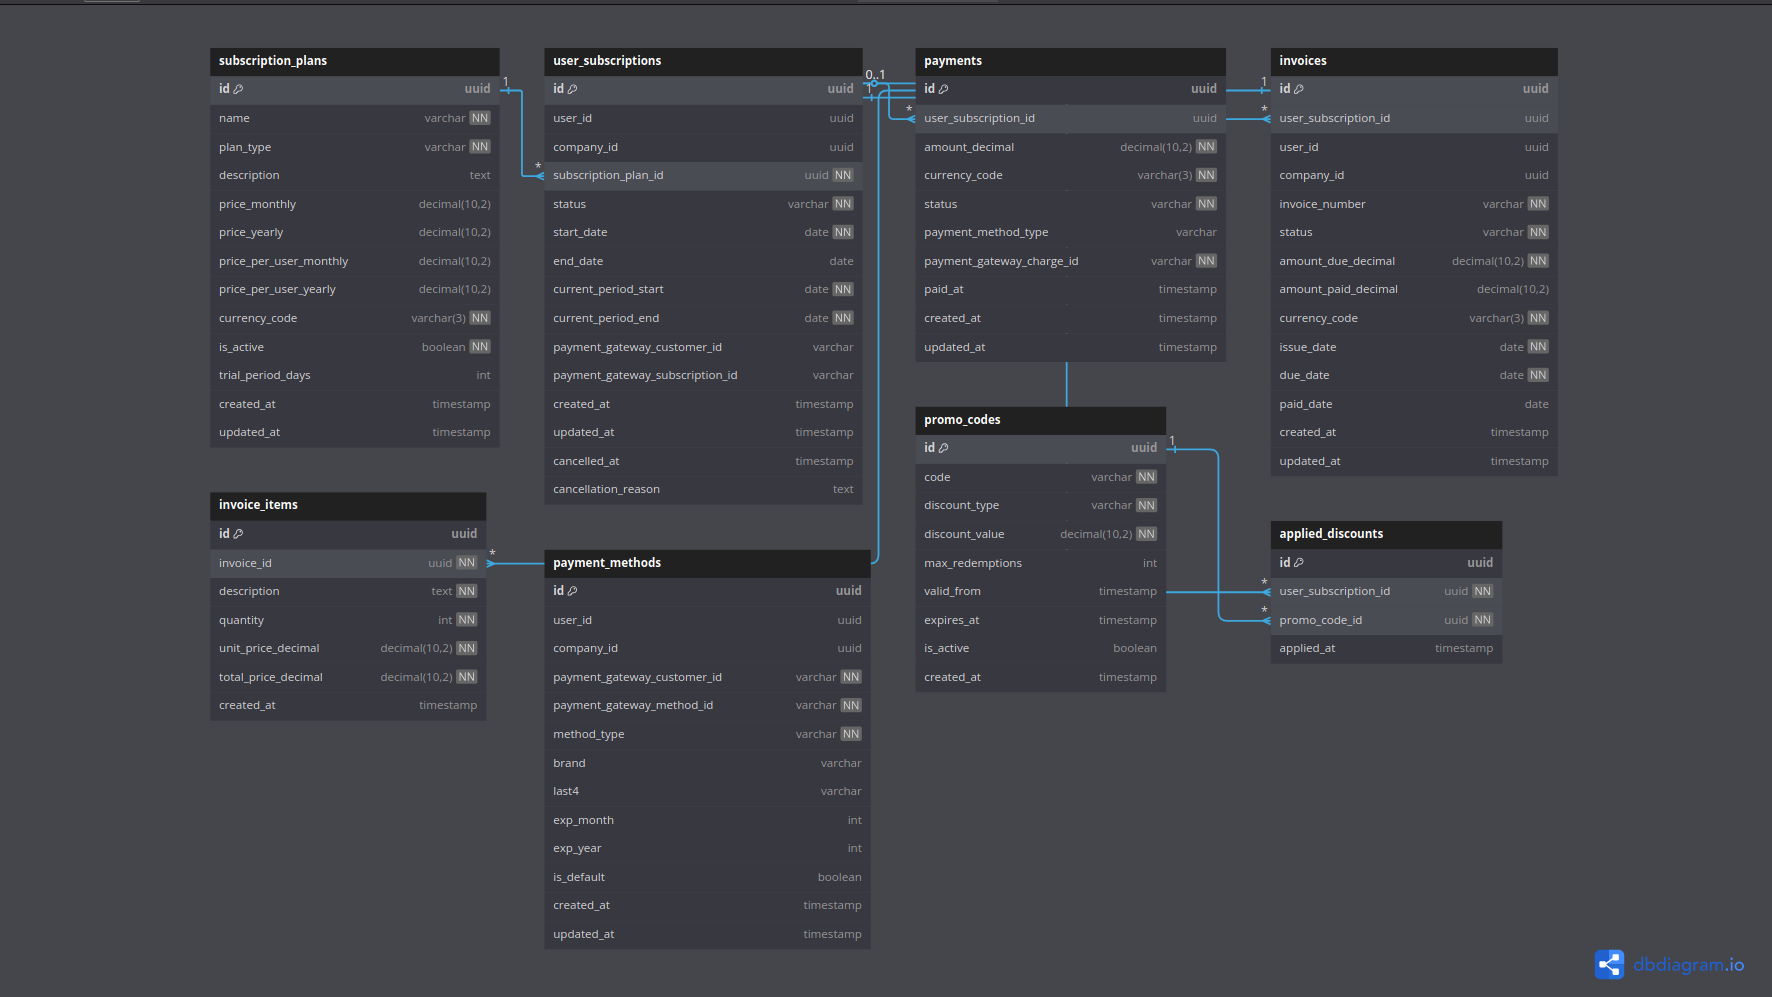
\includegraphics[width=0.8\textwidth,keepaspectratio]{services_db_screanshots/Screenshot 2025-06-06 at 15-05-28 Billing_and_Subscription_Service.pdf.png}
  \caption{\textbf{Modèle de données du service de facturation} pour la gestion des abonnements et des paiements.}
  \label{fig:billing_service}
\end{figure}
\vspace{-10pt}
\small
\paragraph{Points clés du service de Facturation :}
\begin{itemize}[leftmargin=*,noitemsep,topsep=0pt]
  \item \textbf{Gestion des plans d'abonnement} avec différents niveaux de service
  \item \textbf{Suivi des factures et paiements} pour les utilisateurs individuels et entreprises
  \item \textbf{Support des promotions et réductions} temporaires ou permanentes
  \item \textbf{Historique de facturation} complet pour analyses financières
  \item \textbf{Intégration} avec les passerelles de paiement externes
\end{itemize}
\normalsize
\newpage

\subsubsection{Service de Certification}
\begin{figure}[h!]
  \centering
  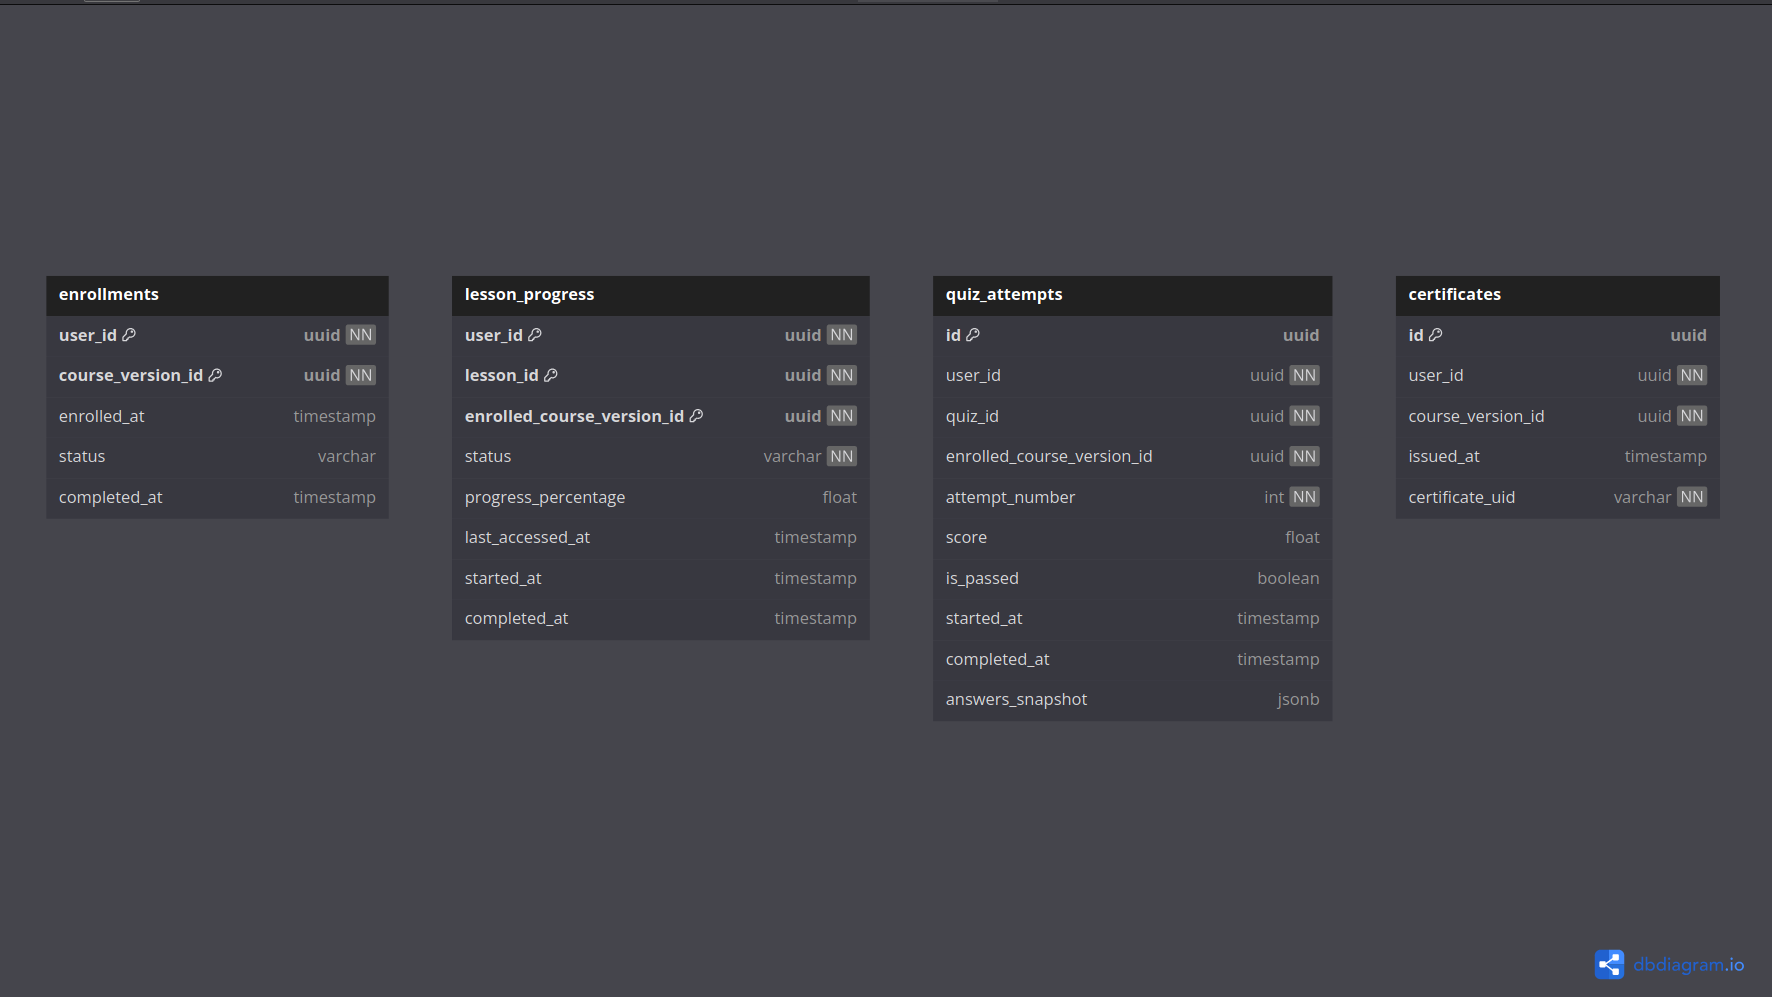
\includegraphics[width=0.8\textwidth,keepaspectratio]{services_db_screanshots/Screenshot 2025-06-06 at 15-05-53 Certification_Service.pdf.png}
  \caption{\textbf{Modèle de données du service de certification} pour la délivrance et la validation des certificats.}
  \label{fig:certification_service}
\end{figure}
\vspace{-10pt}
\small
\paragraph{Points clés du service de Certification :}
\begin{itemize}[leftmargin=*,noitemsep,topsep=0pt]
  \item \textbf{Création de certificats} à l'achèvement des cours et modules
  \item \textbf{Validation et vérification} des compétences acquises
  \item \textbf{Badges et récompenses} pour motiver les apprenants
  \item \textbf{Système de validation externe} permettant aux entreprises de vérifier l'authenticité
  \item \textbf{Historique des certifications} pour chaque utilisateur
\end{itemize}
\normalsize
\newpage

\subsubsection{Service d'Analytique et Reporting}
\begin{figure}[h!]
  \centering
  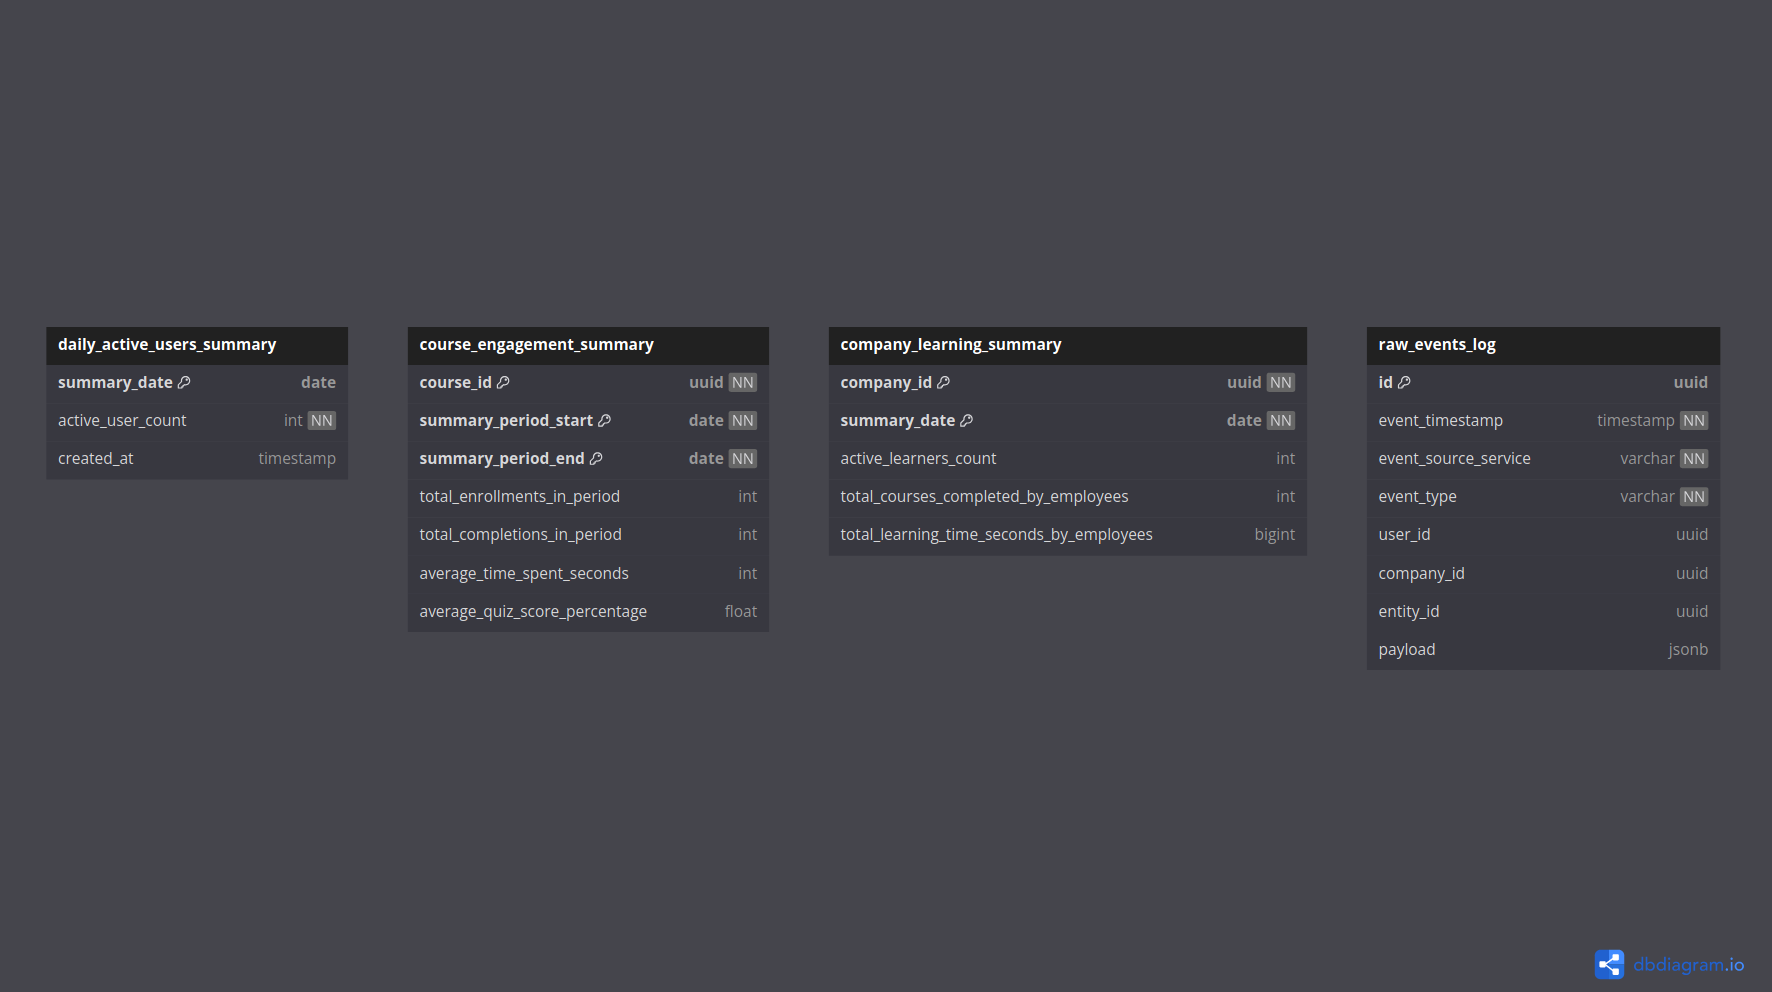
\includegraphics[width=0.8\textwidth,keepaspectratio]{services_db_screanshots/Screenshot 2025-06-06 at 15-04-59 Analytics_and_Reporting_Service.pdf.png}
  \caption{\textbf{Modèle de données du service d'analytique} pour le suivi des performances et la génération de rapports.}
  \label{fig:analytics_service}
\end{figure}
\vspace{-10pt}
\small
\paragraph{Points clés du service d'Analytique :}
\begin{itemize}[leftmargin=*,noitemsep,topsep=0pt]
  \item \textbf{Collecte de données d'utilisation} sur toutes les interactions utilisateurs
  \item \textbf{Métriques de performance} pour les cours et modules
  \item \textbf{Rapports personnalisés} pour les administrateurs et entreprises
  \item \textbf{Tableaux de bord en temps réel} pour le suivi des indicateurs clés
  \item \textbf{Système d'alerte} pour identifier les anomalies ou opportunités
\end{itemize}
\normalsize
\newpage

\subsubsection{Service de Feedback}
\begin{figure}[h!]
  \centering
  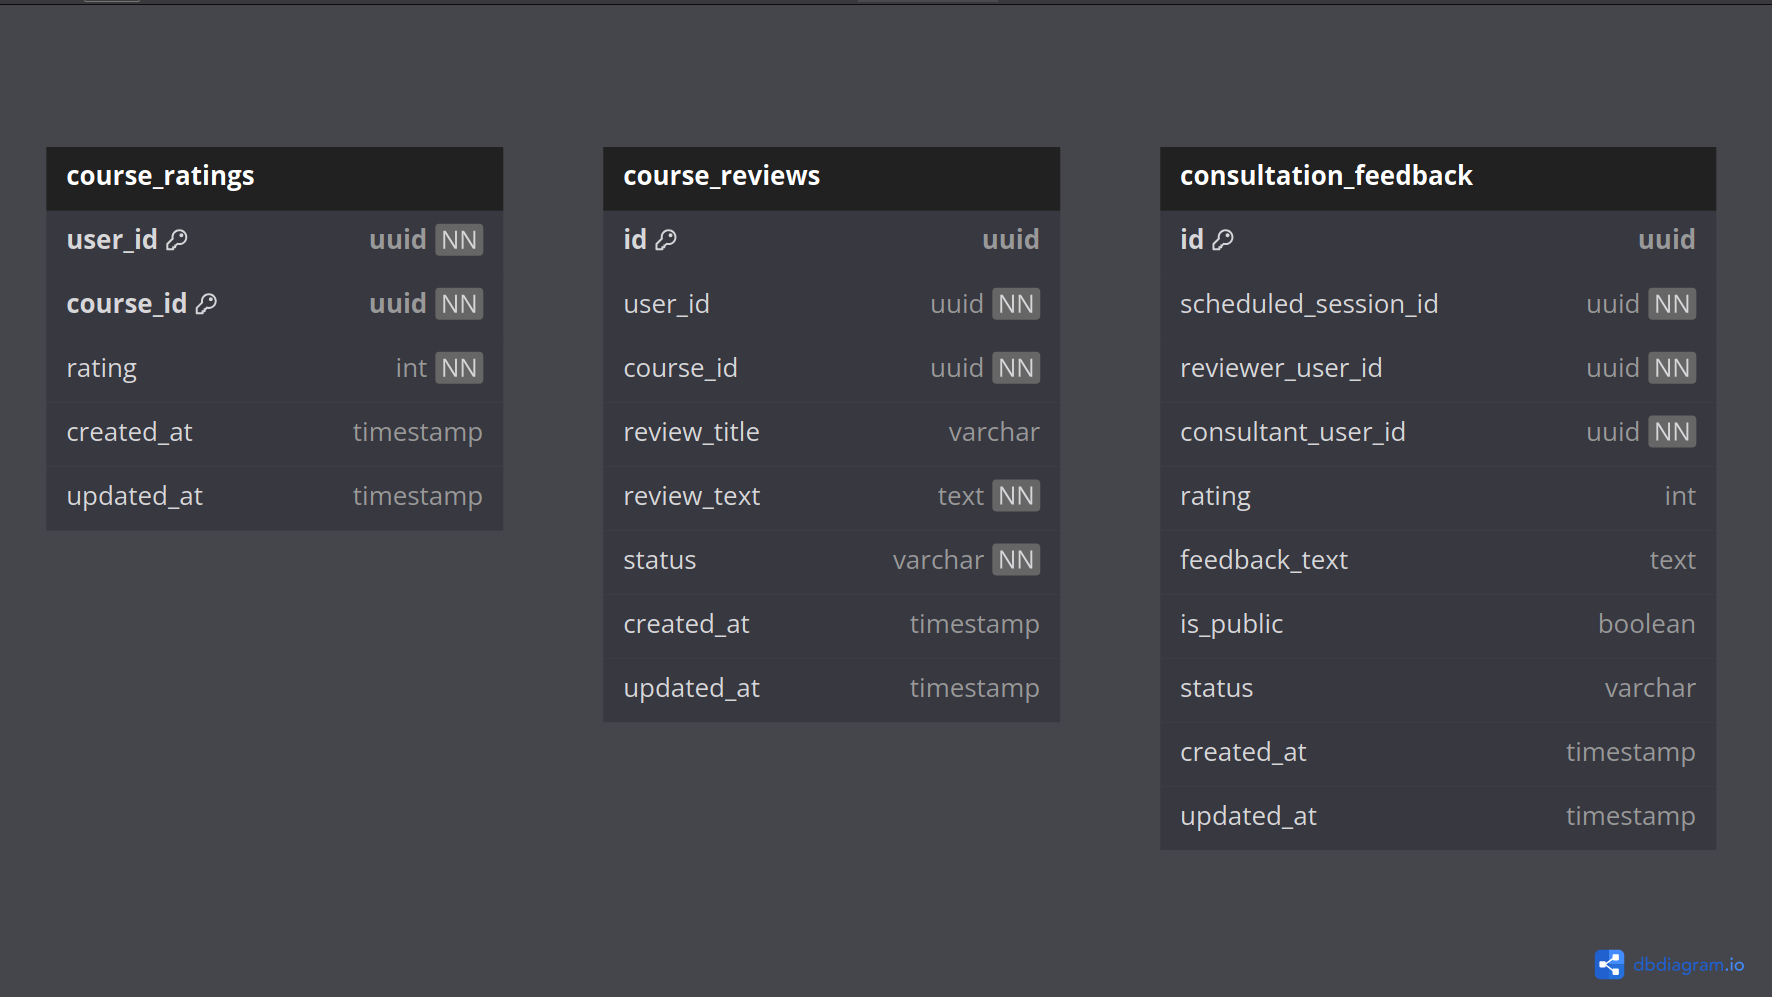
\includegraphics[width=0.8\textwidth,keepaspectratio]{services_db_screanshots/Screenshot 2025-06-06 at 15-08-00 Feedback_Service.pdf.png}
  \caption{\textbf{Modèle de données du service de feedback} pour la collecte et la gestion des retours utilisateurs.}
  \label{fig:feedback_service}
\end{figure}
\vspace{-10pt}
\small
\paragraph{Points clés du service de Feedback :}
\begin{itemize}[leftmargin=*,noitemsep,topsep=0pt]
  \item \textbf{Évaluations et avis} sur les cours et modules
  \item \textbf{Système de notation} permettant une évaluation quantitative
  \item \textbf{Commentaires et suggestions} pour améliorer le contenu
  \item \textbf{Analyse de sentiment} sur les retours textuels
  \item \textbf{Boucle de rétroaction} pour les créateurs de contenu
\end{itemize}
\normalsize
\newpage

\subsubsection{Service de Notification}
\begin{figure}[h!]
  \centering
  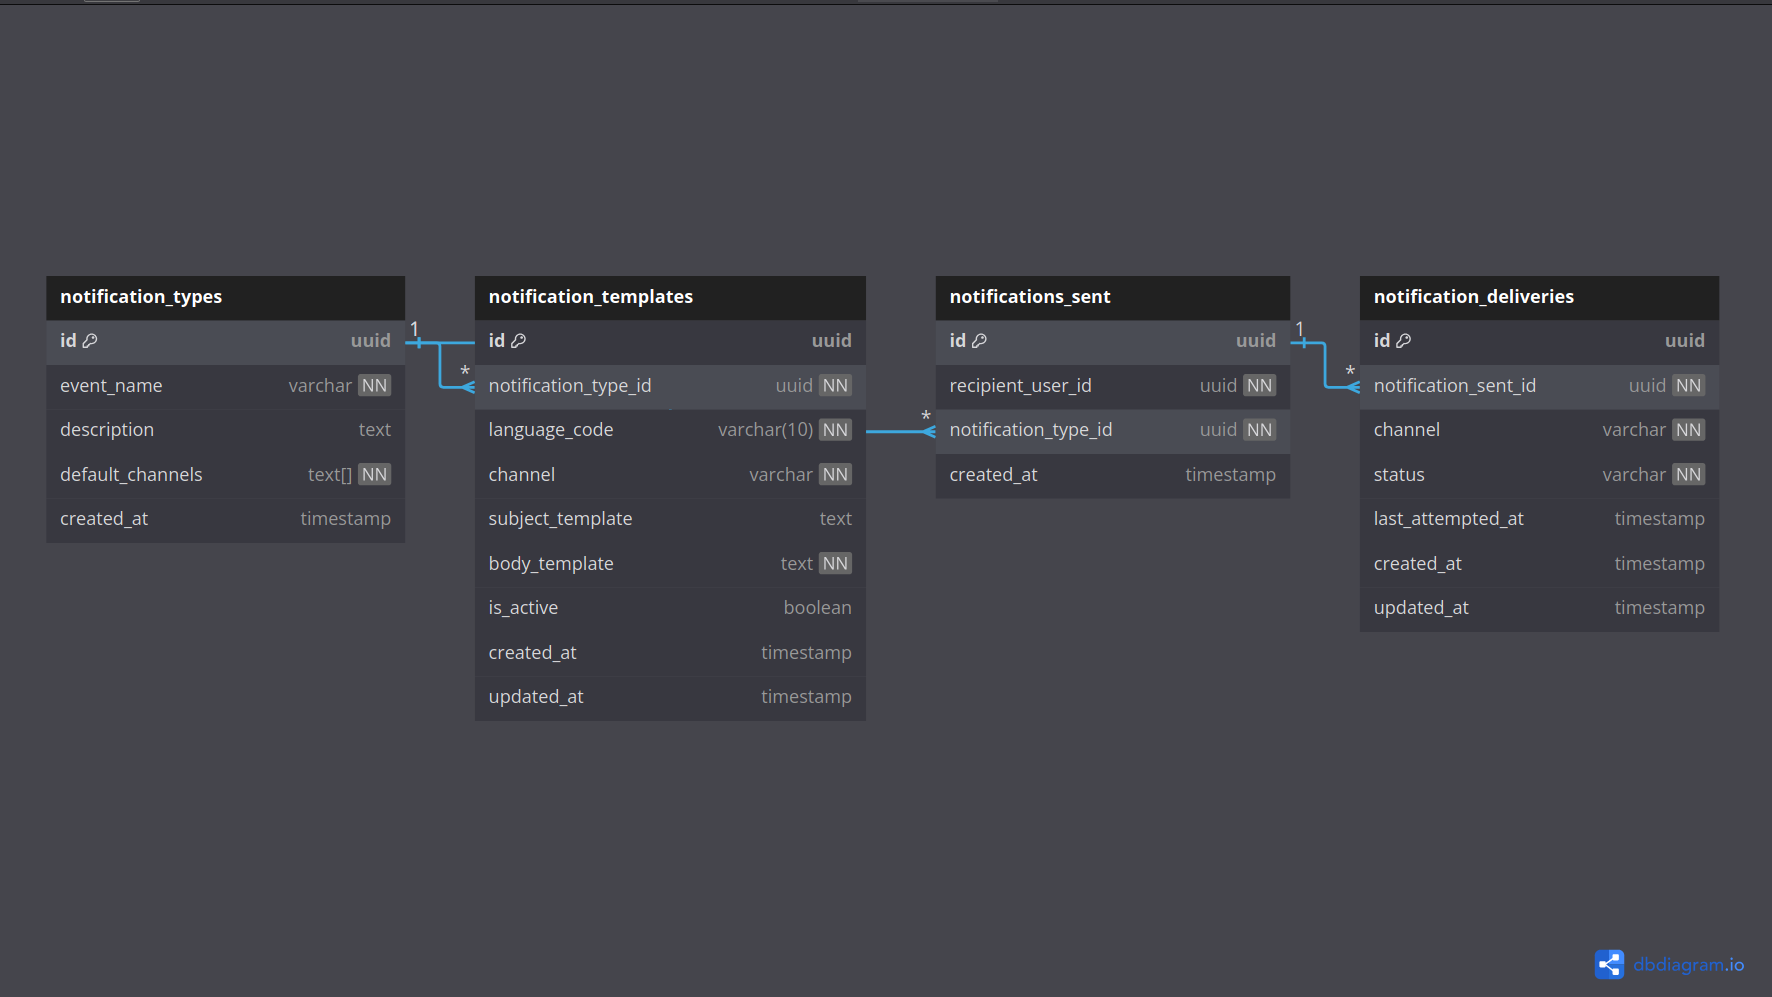
\includegraphics[width=0.8\textwidth,keepaspectratio]{services_db_screanshots/Screenshot 2025-06-06 at 15-08-13 Notification_Service.pdf.png}
  \caption{\textbf{Modèle de données du service de notification} pour l'envoi et la gestion des notifications.}
  \label{fig:notification_service}
\end{figure}
\vspace{-10pt}
\small
\paragraph{Points clés du service de Notification :}
\begin{itemize}[leftmargin=*,noitemsep,topsep=0pt]
  \item \textbf{Notifications temps réel} pour les événements importants
  \item \textbf{Préférences de notification} configurables par utilisateur
  \item \textbf{Support multi-canal} : email, push, in-app, SMS
  \item \textbf{Modèles de messages} personnalisables
  \item \textbf{Planification et automatisation} des campagnes de notification
\end{itemize}
\normalsize
\newpage

\subsubsection{Service de Gestion des Médias}
\begin{figure}[h!]
  \centering
  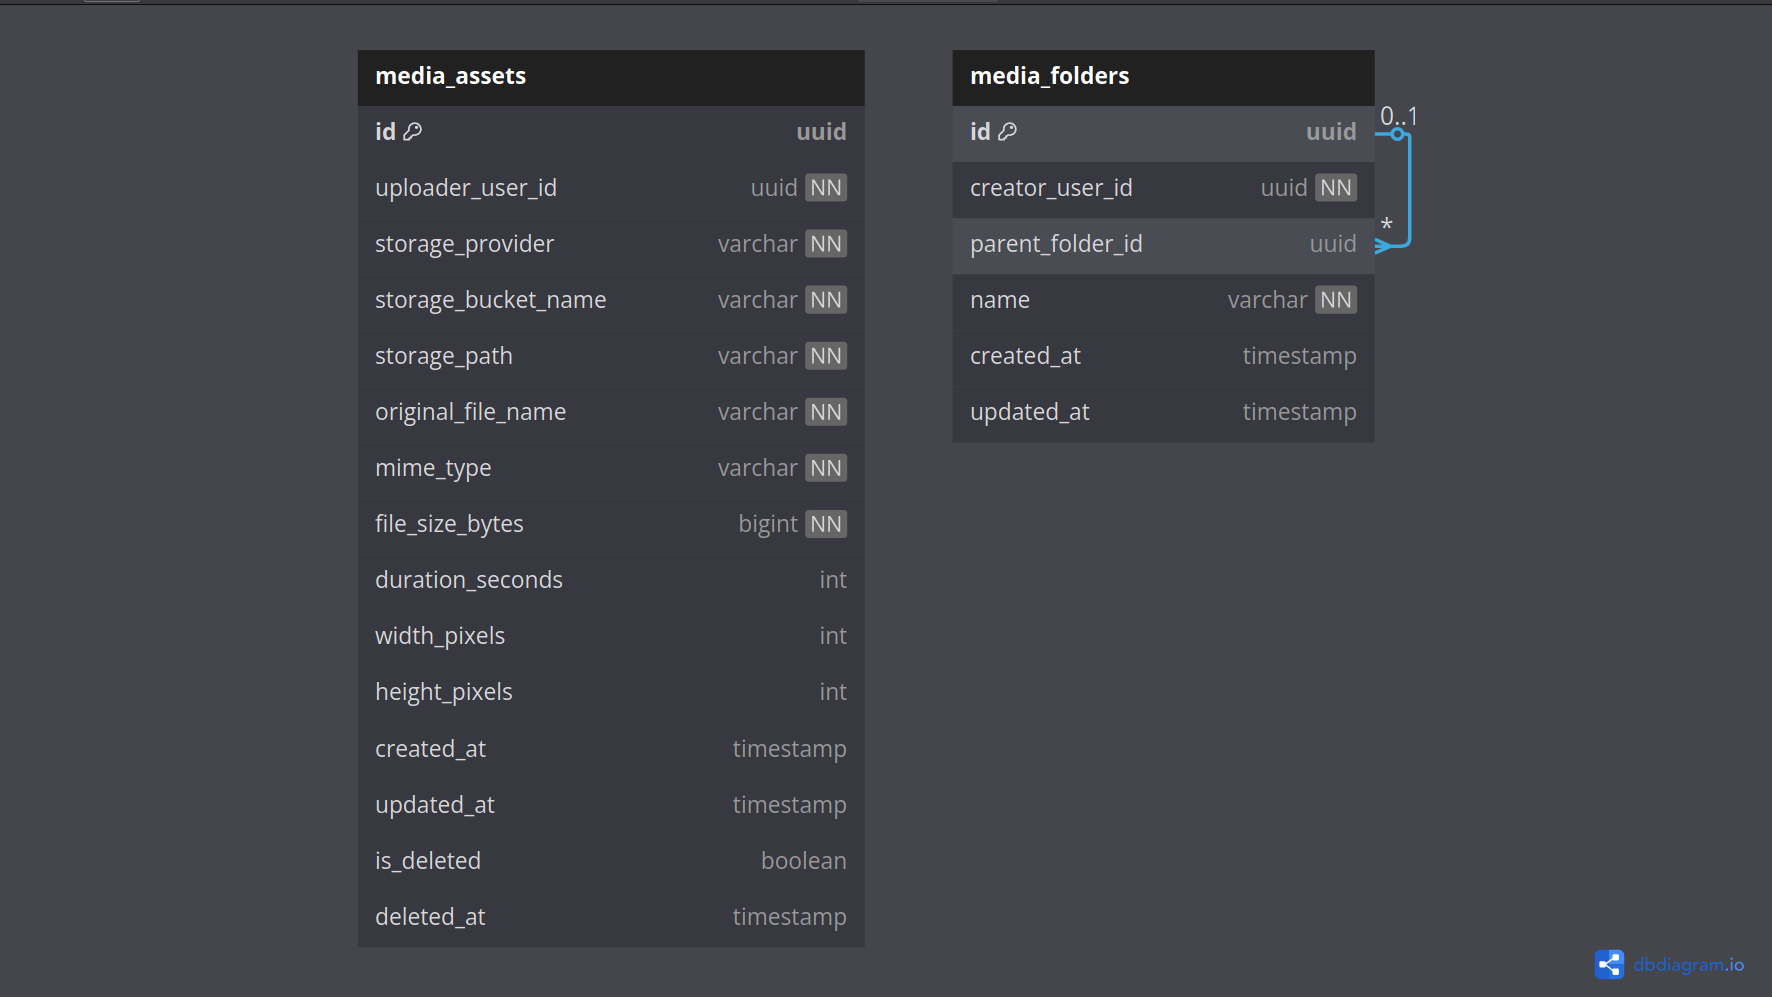
\includegraphics[width=0.8\textwidth,keepaspectratio]{services_db_screanshots/Screenshot 2025-06-06 at 15-08-27 Media_Management_Service.pdf.png}
  \caption{\textbf{Modèle de données du service de gestion des médias} pour le stockage et l'accès aux ressources multimédias.}
  \label{fig:media_service}
\end{figure}
\vspace{-10pt}
\small
\paragraph{Points clés du service de Médias :}
\begin{itemize}[leftmargin=*,noitemsep,topsep=0pt]
  \item \textbf{Gestion centralisée} des ressources audio, vidéo et images
  \item \textbf{Métadonnées enrichies} pour faciliter la recherche et l'organisation
  \item \textbf{Support de multiples formats} et résolutions
  \item \textbf{Optimisation automatique} pour différents appareils
  \item \textbf{Contrôle des droits d'accès} pour les ressources protégées
\end{itemize}
\normalsize
\newpage

\subsubsection{Service de Configuration de la Plateforme}
\begin{figure}[h!]
  \centering
  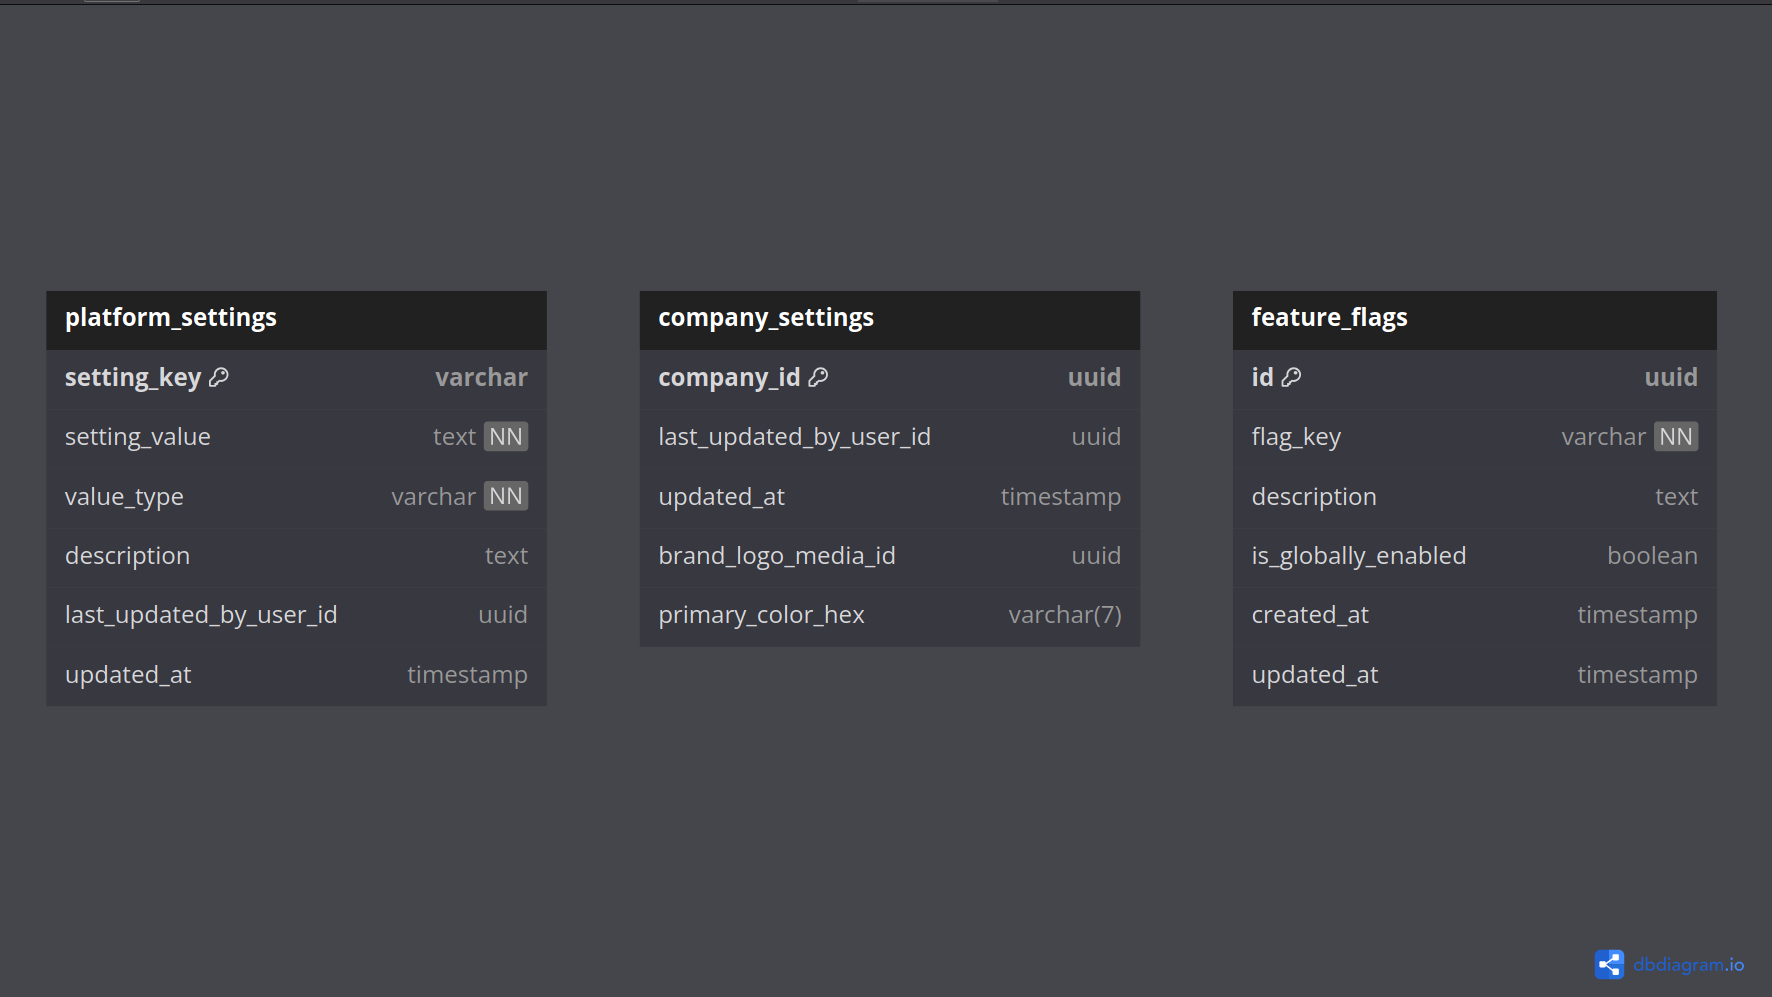
\includegraphics[width=0.8\textwidth,keepaspectratio]{services_db_screanshots/Screenshot 2025-06-06 at 15-08-44 Platform_Configuration_Service.pdf.png}
  \caption{\textbf{Modèle de données du service de configuration} pour la gestion des paramètres globaux de la plateforme.}
  \label{fig:platform_config_service}
\end{figure}
\vspace{-10pt}
\small
\paragraph{Points clés du service de Configuration :}
\begin{itemize}[leftmargin=*,noitemsep,topsep=0pt]
  \item \textbf{Paramètres système} centralisés et accessibles à tous les services
  \item \textbf{Gestion des drapeaux de fonctionnalités} (feature flags)
  \item \textbf{Configuration par environnement} (développement, test, production)
  \item \textbf{Personnalisation de l'interface} selon les besoins spécifiques
  \item \textbf{Paramètres multilingues} pour localisation de la plateforme
\end{itemize}
\normalsize
\newpage

\subsubsection{Service de Recherche}
\begin{figure}[h!]
  \centering
  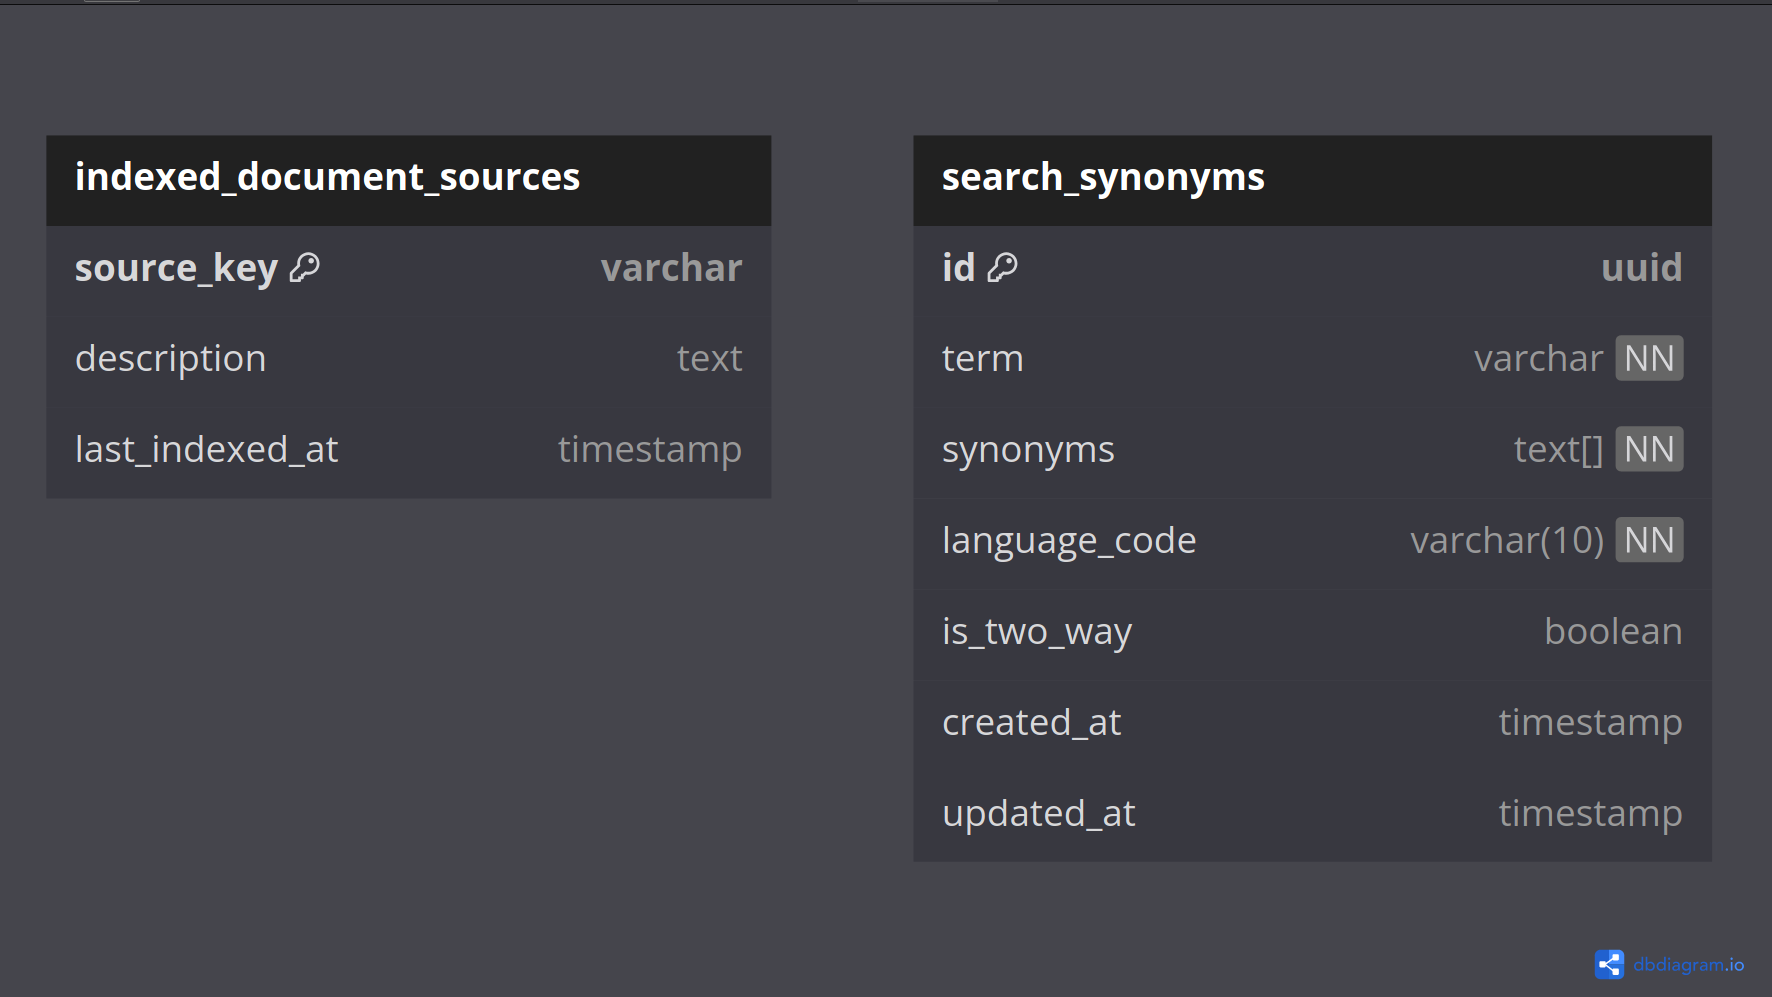
\includegraphics[width=0.8\textwidth,keepaspectratio]{services_db_screanshots/Screenshot 2025-06-06 at 15-08-52 Search_Service.pdf.png}
  \caption{\textbf{Modèle de données du service de recherche} pour l'indexation et la recherche de contenu.}
  \label{fig:search_service}
\end{figure}
\vspace{-10pt}
\small
\paragraph{Points clés du service de Recherche :}
\begin{itemize}[leftmargin=*,noitemsep,topsep=0pt]
  \item \textbf{Indexation intelligente} du contenu des cours et ressources
  \item \textbf{Recherche full-text} avec prise en charge des synonymes
  \item \textbf{Système de tags} pour améliorer la pertinence des résultats
  \item \textbf{Historique des recherches} pour l'analyse des tendances
  \item \textbf{Algorithme de recommandation} basé sur les comportements de recherche
\end{itemize}

\begin{table}[h!]
\centering
\small
\caption{Comparaison des caractéristiques techniques des services}
\label{tab:comparaison_services}
\begin{tabular}{|l|c|c|c|}
\hline
\textbf{Service} & \textbf{Technologie principale} & \textbf{Type de données} & \textbf{Complexité} \\
\hline
IAM & Node.js/Go & Utilisateurs & Élevée \\
Contenu & Python/FastAPI & Éducation & Moyenne \\
Facturation & Python/FastAPI & Financières & Élevée \\
Certification & Python/Go & Validation & Moyenne \\
Analytique & Python & Statistiques & Élevée \\
Feedback & Node.js & Évaluation & Basse \\
Notification & Go & Messaging & Moyenne \\
Médias & Node.js & Binaires & Élevée \\
Configuration & Go & Paramètres & Basse \\
Recherche & Python/Elasticsearch & Index & Élevée \\
\hline
\end{tabular}
\end{table}
\normalsize 

% Chapter 4: Development and Implementation
\chapter*{Chapitre 4 : Réalisation et mise en pied du système}
\addcontentsline{toc}{chapter}{Chapitre 4 : Réalisation et mise en pied du système}
\thispagestyle{fancy}
\setcounter{section}{0}
\newpage

\section{Outils et technologies de développement}
Pour le développement du projet, plusieurs outils et technologies modernes ont été utilisés afin d'assurer la qualité, la performance et la maintenabilité du code.

\subsection{Environnement de développement}
L'environnement de développement a été configuré avec les outils suivants :
\begin{itemize}
  \item \textbf{Visual Studio code et neovim :} Comme éditeur de code principaux avec des extensions pour React, TypeScript et ESLint
  \item \textbf{GitHub :} Pour la gestion de versions et la collaboration
  \item \textbf{Docker :} Pour la conteneurisation des services backend
  \item \textbf{Postman :} Pour tester les API
  \item \textbf{Chrome DevTools :} Pour le debugging et l'optimisation des performances frontend
\end{itemize}

\subsection{Technologies frontend}
Pour le développement front-end de cette application, les technologies suivantes ont été utilisées :
\begin{itemize}
  \item \textbf{Next.js :} Framework React pour le rendu côté serveur et la génération de sites statiques
  \item \textbf{Tailwind CSS :} Framework CSS utilitaire pour un design responsive et personnalisable
  \item \textbf{Framer Motion :} Bibliothèque d'animations pour ajouter des transitions et effets visuels
  \item \textbf{React Hook Form :} Gestion des formulaires avec validation
  \item \textbf{TypeScript :} Pour un code plus robuste avec typage statique
\end{itemize}

\subsection{Technologies backend}
Pour le développement backend, les technologies suivantes ont été utilisées :
\begin{itemize}
  \item \textbf{Node.js :} Environnement d'exécution JavaScript côté serveur
  \item \textbf{Express :} Framework web pour Node.js
  \item \textbf{PostgreSQL :} Système de gestion de base de données relationnelle
  \item \textbf{Supabase :} Plateforme Backend-as-a-Service pour l'authentification et le stockage
  \item \textbf{Redis :} Pour la mise en cache et la gestion des sessions
\end{itemize}



% Chapter 5: Deployment and Optimization
% \chapter{Chapitre 5 : Déploiement et Tests}
\thispagestyle{fancy}
\newpage

La troisième semaine du stage a été consacrée au développement des interfaces utilisateur pour la plateforme d'apprentissage en ligne, ainsi qu'à la mise en place d'un système avancé de traitement des données de contenu. Ces avancées ont permis de construire les fondations interactives de la plateforme et d'optimiser le traitement des ressources pédagogiques.

\section{Intégration et Déploiement du Backend}

La phase de déploiement a impliqué la mise en place de l'infrastructure nécessaire pour héberger et exécuter la plateforme en environnement de production.

\subsection{Configuration du Serveur}

La configuration du serveur a été réalisée en suivant les meilleures pratiques de sécurité et de performance. Les étapes principales ont inclus :

\begin{itemize}
  \item Installation et configuration du système d'exploitation (Linux Ubuntu Server)
  \item Mise en place des règles de pare-feu et de sécurité
  \item Configuration des certificats SSL pour assurer des connexions sécurisées
  \item Installation des dépendances nécessaires au fonctionnement de l'application
  \item Configuration des services de monitoring et de logging
\end{itemize}

\subsection{Déploiement de la Base de Données}

Pour assurer une accessibilité optimale et une scalabilité future, la base de données a été déployée sur MongoDB Atlas, une plateforme de base de données en tant que service (DBaaS). Cette solution cloud offre plusieurs avantages :

\begin{itemize}
  \item Haute disponibilité avec réplication automatique
  \item Surveillance en temps réel des performances
  \item Sauvegardes automatisées
  \item Sécurité renforcée avec authentification et chiffrement
  \item Scalabilité horizontale et verticale selon les besoins
\end{itemize}

\begin{figure}[h!]
  \centering
  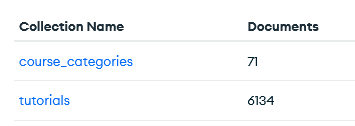
\includegraphics[width=0.9\textwidth,keepaspectratio]{week_3_img/Screenshot 2025-05-19 234047.png}
  \caption{\textbf{Interface MongoDB Atlas} montrant les différentes collections de données.}
  \label{fig:mongodb_collections}
\end{figure}

\subsection{Évolution de l'Architecture}

Après des tests approfondis, une décision stratégique a été prise de migrer d'une architecture MongoDB vers une solution basée sur des fichiers JSON locaux. Cette transition a été motivée par :

\begin{itemize}
  \item La réduction de la complexité architecturale pour la phase actuelle du projet
  \item L'amélioration de l'expérience de développement avec un accès direct aux données
  \item La compatibilité optimale avec le framework Next.js et ses capacités de rendu côté serveur
  \item La simplification du déploiement et de la maintenance pour les premiers stades du projet
\end{itemize}

\section{Intégration et Tests}

\subsection{Tests Unitaires}

Une suite de tests unitaires a été développée pour valider le bon fonctionnement des différents composants de l'application :

\begin{itemize}
  \item Tests des modèles de données
  \item Tests des contrôleurs et services
  \item Tests des utilitaires et fonctions auxiliaires
  \item Tests des composants React avec Jest et React Testing Library
\end{itemize}

\subsection{Tests d'Intégration}

Des tests d'intégration ont été mis en place pour vérifier les interactions entre les différents modules de l'application :

\begin{itemize}
  \item Tests des flux de données entre le frontend et le backend
  \item Tests des interactions avec la base de données
  \item Tests des flux d'authentification et d'autorisation
  \item Tests des processus métier complets
\end{itemize}

\subsection{Tests de Performance}

Des tests de performance ont été réalisés pour s'assurer que l'application répond aux exigences en termes de temps de réponse et de capacité à gérer la charge :

\begin{itemize}
  \item Tests de charge avec simulation d'utilisateurs concurrents
  \item Tests de stress pour identifier les limites de l'application
  \item Analyse des goulots d'étranglement et optimisations nécessaires
  \item Mesure des temps de chargement des pages et des composants
\end{itemize}

\section{Optimisation et Monitoring}

\subsection{Optimisation des Performances}

Plusieurs optimisations ont été apportées pour améliorer les performances de l'application :

\begin{itemize}
  \item Intégration des capacités de rendu côté serveur de Next.js pour améliorer les performances perçues
  \item Mise en place de stratégies de mise en cache pour les données fréquemment accédées
  \item Optimisation des images et des ressources statiques
  \item Implémentation du lazy loading pour les composants non critiques
  \item Minification et bundling des fichiers JavaScript et CSS
\end{itemize}

\subsection{Mise en Place du Monitoring}

Un système de monitoring a été mis en place pour surveiller l'état et les performances de l'application en production :

\begin{itemize}
  \item Intégration de Sentry pour la détection et le suivi des erreurs
  \item Configuration de New Relic pour le monitoring des performances
  \item Mise en place de dashboards de monitoring avec Grafana
  \item Configuration d'alertes en cas de problèmes critiques
  \item Centralisation des logs pour faciliter le débogage
\end{itemize}

\subsection{Documentation}

Une documentation complète a été rédigée pour faciliter la maintenance et l'évolution future de l'application :

\begin{itemize}
  \item Documentation technique de l'architecture
  \item Documentation des API et des endpoints
  \item Guide de déploiement et d'administration
  \item Documentation utilisateur pour les administrateurs de la plateforme
  \item Documentation du processus de développement et des standards de code
\end{itemize}

\section{Conception et Développement de l'Interface Utilisateur}

Après avoir développé la page d'accueil la semaine précédente, l'accent a été mis sur la création des interfaces principales que les utilisateurs utiliseront quotidiennement pour accéder aux contenus et suivre leur progression.

\subsection{Interface d'Accueil des Utilisateurs Connectés}

Une interface d'accueil spécifique pour les utilisateurs connectés a été développée, offrant un accès rapide aux cours en cours, aux recommandations personnalisées et aux dernières activités.

\begin{figure}[h!]
  \centering
  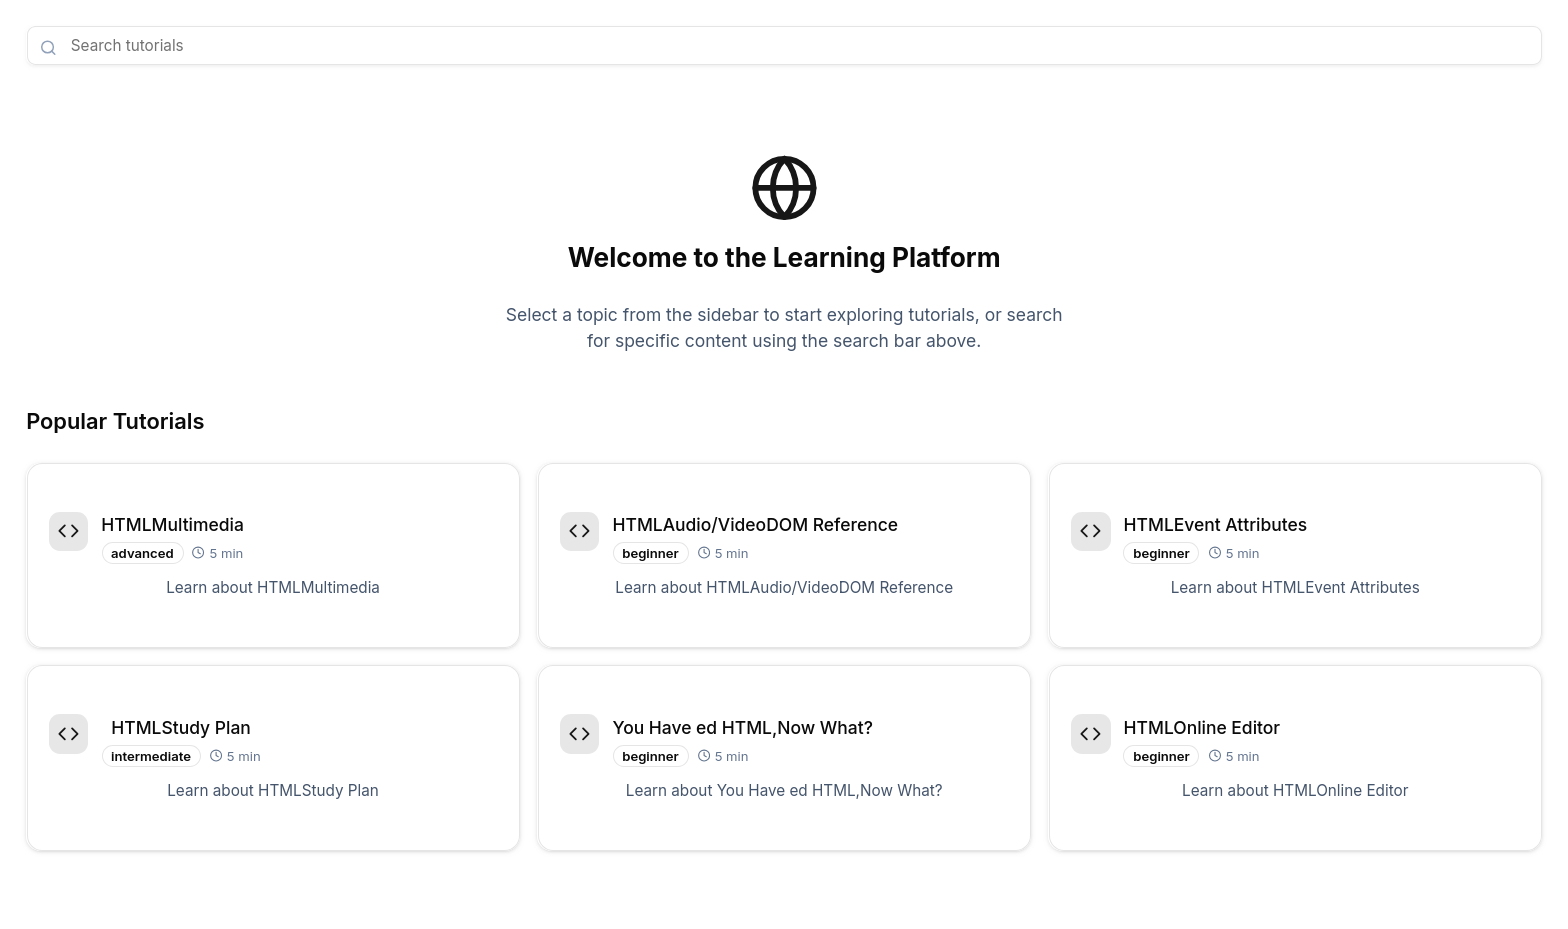
\includegraphics[width=0.9\textwidth,keepaspectratio]{week_3_img/accueil.png}
  \caption{\textbf{Interface d'accueil personnalisée} pour les utilisateurs connectés.}
  \label{fig:user_dashboard}
\end{figure}

\subsection{Barre Latérale de Navigation}

Une barre latérale de navigation intuitive a été implémentée pour faciliter l'accès aux différentes sections de la plateforme.

\begin{figure}[h!]
  \centering
  
\includegraphics[width=0.4\textwidth,keepaspectratio]{week_3_img/sidebare.png}
  \caption{\textbf{Barre latérale de navigation} avec accès aux principales fonctionnalités.}
  \label{fig:sidebar_nav}
\end{figure}

Cette barre latérale comprend :
\begin{itemize}
  \item Accès au tableau de bord personnel
  \item Catalogue de cours et formations
  \item Suivi de progression
  \item Calendrier des sessions de consultation
  \item Paramètres du compte
  \item Centre de notifications
\end{itemize}

\subsection{Interface de Consultation des Cours}

L'interface de consultation des cours a été conçue pour offrir une expérience d'apprentissage immersive et efficace.

\begin{figure}[h!]
  \centering
  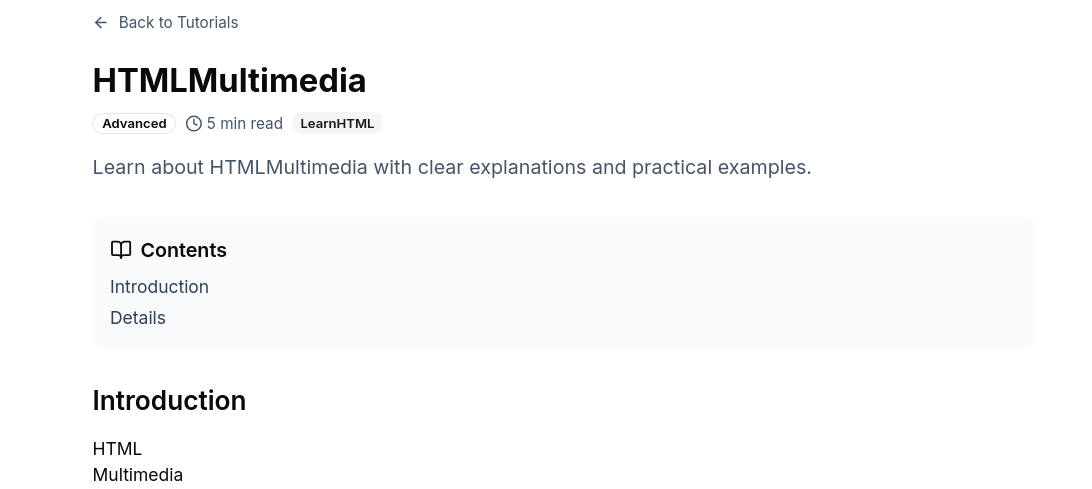
\includegraphics[width=0.9\textwidth,keepaspectratio]{week_3_img/part1.png}
  \caption{\textbf{Interface de consultation des cours} - Partie théorique.}
  \label{fig:course_view_part1}
\end{figure}

\begin{figure}[h!]
  \centering
  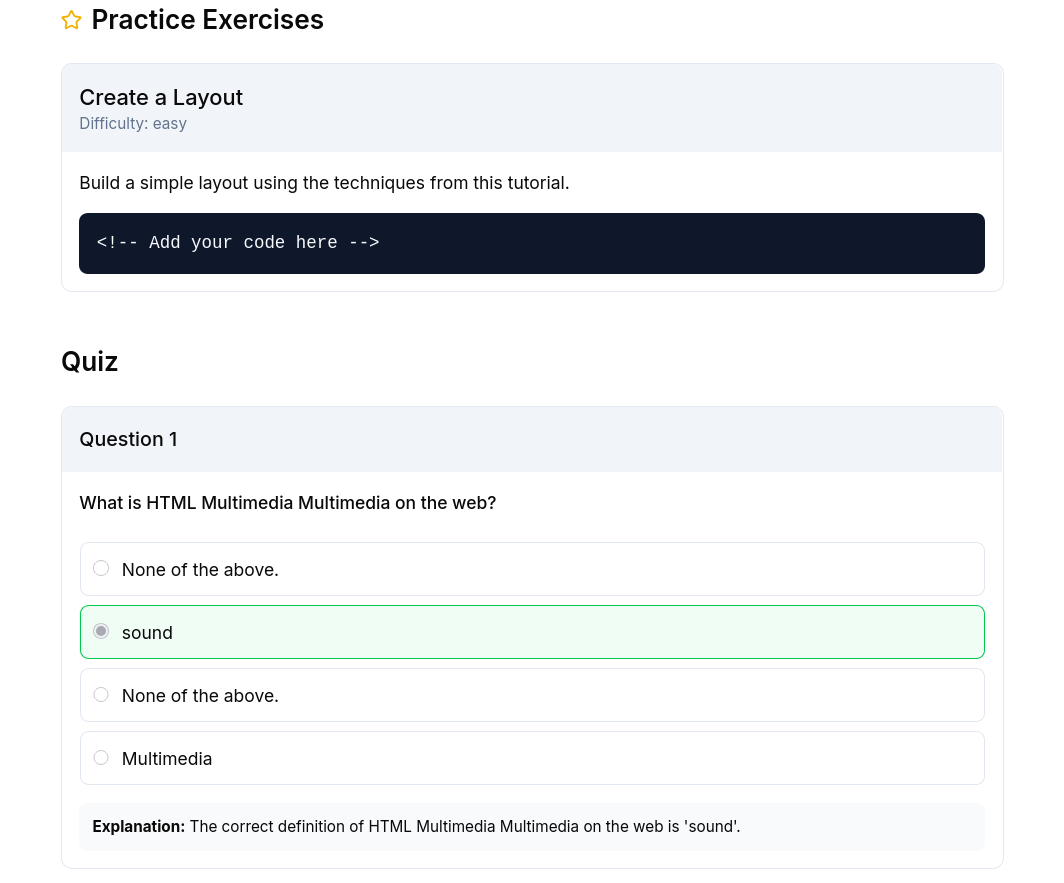
\includegraphics[width=0.9\textwidth,keepaspectratio]{week_3_img/part2.png}
  \caption{\textbf{Interface de consultation des cours} - Partie pratique avec exercices interactifs.}
  \label{fig:course_view_part2}
\end{figure}

Les caractéristiques principales de cette interface incluent :
\begin{itemize}
  \item Affichage clair du contenu théorique avec mise en forme optimisée
  \item Navigation intuitive entre les différentes sections du cours
  \item Exercices interactifs intégrés directement dans l'interface
  \item Suivi de progression en temps réel
  \item Possibilité de prendre des notes contextuelles
  \item Mode sombre/clair pour améliorer le confort de lecture
\end{itemize}

\section{Traitement Avancé des Données de Contenu}

Une partie importante de cette semaine a été consacrée à l'optimisation du traitement des données de contenu éducatif.

\subsection{Défis du Traitement des Données}

Le traitement des données collectées présentait plusieurs défis :
\begin{itemize}
  \item Distinction entre le contenu textuel explicatif et les exemples de code
  \item Structuration cohérente des exemples et exercices
  \item Préservation des formatages spécifiques (tableaux, listes, etc.)
  \item Gestion des caractères spéciaux et encodages
  \item Extraction des métadonnées pertinentes
\end{itemize}

\subsection{Problématique du Scraping et Nettoyage des Données}

L'un des défis majeurs rencontrés a été la séparation du contenu textuel explicatif et des extraits de code dans les sections détaillées des cours. Plusieurs approches ont été explorées :

\begin{itemize}
  \item Tentatives initiales avec des expressions régulières et des algorithmes de traitement de texte, atteignant une précision maximale de 80\%
  \item Expérimentation avec un agent IA basé sur des modèles de langage large (LLM) pour effectuer cette séparation de manière plus intelligente
  \item Découverte finale que la structure HTML particulière de W3Schools nécessitait une approche de scraping spécifique
\end{itemize}

La solution définitive a impliqué une refonte du script de scraping pour mieux cibler les éléments HTML spécifiques, permettant ainsi d'obtenir des données brutes de meilleure qualité dès le départ.

\subsection{Implémentation d'un Pipeline de Traitement LLM}

Pour surmonter ces défis, un pipeline de traitement basé sur des modèles de langage large (LLM) a été conçu et implémenté.

\begin{figure}[h!]
  \centering
  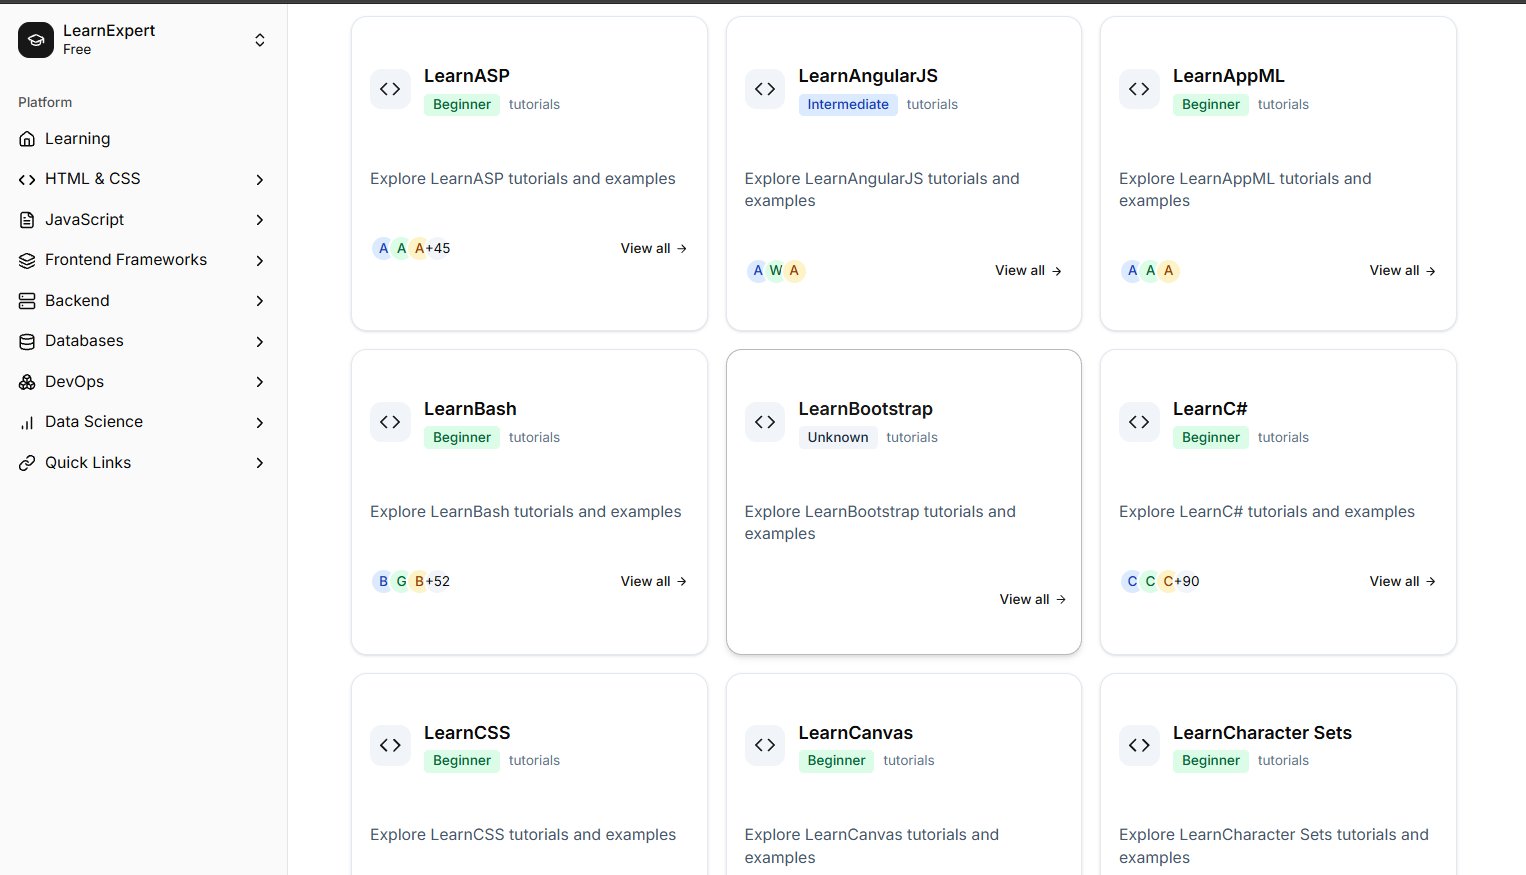
\includegraphics[width=0.9\textwidth,keepaspectratio]{week_3_img/Screenshot 2025-05-20 164411.png}
  \caption{\textbf{Interface d'administration du pipeline LLM} montrant les statistiques de traitement.}
  \label{fig:llm_pipeline}
\end{figure}

\subsection{Stratégie d'Optimisation Multi-LLM}

Le traitement initial utilisant un LLM unique ayant démontré une excellente précision mais des performances limitées en termes de vitesse, une stratégie d'optimisation a été mise en place :

\begin{itemize}
  \item \textbf{Utilisation simultanée de plusieurs fournisseurs LLM :} Parallélisation des requêtes vers différentes API
  \item \textbf{Traitement asynchrone :} Optimisation de la latence perçue en traitant plusieurs segments de données simultanément
  \item \textbf{Segmentation intelligente :} Division des données en unités de traitement optimales pour chaque type de modèle
  \item \textbf{Gestion des requêtes :} Assignation statique de segments spécifiques à des modèles dédiés pour simplifier la gestion de la concurrence
\end{itemize}

Cette approche a permis de réduire significativement le temps de traitement tout en maintenant une qualité optimale, passant d'environ 15 heures à 7-8 heures pour l'ensemble des données.

\section{Intégration Frontend-Backend}

Une attention particulière a été portée à l'intégration efficace entre le frontend et le backend de la plateforme.

\subsection{Développement des Routes d'API}

Des routes d'API RESTful ont été développées pour permettre à l'interface utilisateur d'accéder aux données structurées dans MongoDB :

\begin{itemize}
  \item Routes d'authentification et de gestion des utilisateurs
  \item Routes d'accès au catalogue de cours
  \item Routes de suivi de progression
  \item Routes de gestion des consultations et réservations
  \item Routes d'analytics et de rapports
\end{itemize}

\subsection{Optimisation des Requêtes}

Les requêtes MongoDB ont été optimisées pour garantir des performances optimales :

\begin{itemize}
  \item Création d'index appropriés pour accélérer les recherches fréquentes
  \item Limitation des champs retournés aux données strictement nécessaires
  \item Utilisation de projections pour alléger les transferts de données
  \item Mise en place de pagination pour les listes volumineuses
  \item Implémentation de mécanismes de mise en cache pour les données fréquemment consultées
\end{itemize}

\subsection{Adaptation à l'Architecture JSON}

Suite à la migration vers des fichiers JSON locaux, l'architecture d'accès aux données a été adaptée :

\begin{itemize}
  \item Développement de fonctions de récupération (fetch) optimisées pour les fichiers JSON
  \item Mise en place d'un système de chargement dynamique des données pour les différentes sections de l'interface
  \item Intégration des capacités de rendu côté serveur de Next.js pour améliorer les performances
\end{itemize}

Cette adaptation a permis de maintenir toutes les fonctionnalités prévues tout en simplifiant l'architecture globale du système.

\section{Tests et Validation}

Pour garantir la qualité et la fiabilité des interfaces et systèmes développés, plusieurs types de tests ont été mis en place :

\subsection{Tests d'Interface Utilisateur}

\begin{itemize}
  \item \textbf{Tests de compatibilité :} Vérification du rendu sur différents navigateurs (Chrome, Firefox, Safari, Edge)
  \item \textbf{Tests de responsive design :} Validation de l'adaptation aux différentes tailles d'écran
  \item \textbf{Tests d'accessibilité :} Conformité aux standards WCAG pour garantir l'inclusivité
  \item \textbf{Tests d'utilisabilité :} Évaluation de l'intuitivité et de la fluidité de navigation
\end{itemize}

\subsection{Tests Fonctionnels et d'Intégration}

\begin{itemize}
  \item \textbf{Tests des routes d'API :} Validation des entrées/sorties et gestion des erreurs
  \item \textbf{Tests d'intégration :} Vérification de la communication correcte entre frontend et backend
  \item \textbf{Tests de performance :} Mesure des temps de réponse et optimisation des goulots d'étranglement
  \item \textbf{Tests de charge :} Simulation d'utilisation intensive pour évaluer la robustesse
\end{itemize}

\subsection{Planification Stratégique pour l'Avenir}

En fin de semaine, une réflexion stratégique a été menée concernant l'enrichissement du contenu et la différenciation de la plateforme :

\begin{itemize}
  \item Identification du besoin de diversifier les sources de contenu au-delà de W3Schools
  \item Planification de l'intégration d'éléments interactifs avancés, comme un éditeur de code basé sur les technologies VSCode
  \item Initiation à l'apprentissage des techniques d'optimisation pour les moteurs de recherche (SEO) pour améliorer la visibilité future de la plateforme
\end{itemize}

\section{Conclusion}

Cette troisième semaine a marqué des avancées significatives dans le développement de la plateforme e-learning. La mise en place d'interfaces utilisateur intuitives et ergonomiques, couplée à un système sophistiqué de traitement des données éducatives, a permis de poser les fondations solides pour l'expérience utilisateur finale. L'utilisation innovante de technologies comme MongoDB Atlas et les modèles de langage large (LLM) a apporté des solutions efficaces aux défis techniques rencontrés.

Les interfaces développées durant cette semaine offrent maintenant aux utilisateurs un environnement d'apprentissage fluide et immersif, tandis que l'optimisation du traitement des données garantit une qualité exceptionnelle du contenu éducatif proposé. Les décisions stratégiques prises, notamment la simplification de l'architecture de données et la planification d'éléments différenciateurs, posent les bases d'une plateforme compétitive et évolutive. 

% Chapter 6: Assessment and Future Perspectives
% \chapter*{Chapitre 6 : Bilan et Perspectives}
\addcontentsline{toc}{chapter}{Chapitre 6 : Bilan et Perspectives}
\thispagestyle{fancy}
\setcounter{section}{0}
\newpage

Ce chapitre présente un bilan du projet réalisé pendant le stage, les fonctionnalités implémentées, les défis techniques surmontés, ainsi que les perspectives de développement futur de la plateforme LearnExpert.

\section{Réalisations et État Actuel du Projet}

\subsection{Fonctionnalités Implémentées}
Au terme de ce stage de quatre semaines, les fonctionnalités suivantes ont été implémentées avec succès :

\begin{itemize}
  \item \textbf{Architecture de base} : Mise en place d'une architecture microservices robuste et évolutive
  \item \textbf{Site vitrine} : Développement complet du site vitrine avec landing page interactive
  \item \textbf{Système d'authentification} : Implémentation de l'authentification des utilisateurs via Supabase
  \item \textbf{Dashboard utilisateur} : Création d'une interface de tableau de bord personnalisée
  \item \textbf{Éditeur de code interactif} : Intégration d'un éditeur Monaco avec coloration syntaxique et exécution en temps réel
  \item \textbf{Système de navigation} : Développement d'une navigation contextuelle et intuitive
  \item \textbf{Base de données structurée} : Migration des données scrappées et nettoyées vers une structure JSON optimisée
  \item \textbf{Pipeline de traitement de données} : Mise en place d'un système de nettoyage utilisant des modèles LLM
\end{itemize}

Ces réalisations constituent les fondations solides sur lesquelles la plateforme pourra continuer à se développer.

\subsection{Défis Techniques Surmontés}
Plusieurs défis techniques majeurs ont été rencontrés et surmontés au cours du développement :

\begin{itemize}
  \item \textbf{Séparation du code et du texte} : La difficulté initiale à distinguer automatiquement le code explicatif du code exécutable dans les données scrappées a été résolue grâce à l'utilisation innovante de modèles de langage large (LLM) en parallèle.
  
  \item \textbf{Performances de l'éditeur de code} : L'intégration de l'éditeur Monaco dans l'application Next.js a posé des défis de performance qui ont été résolus par une stratégie de chargement dynamique et de mise en cache.
  
  \item \textbf{Cohérence des données} : La gestion de la cohérence des données à travers les différents microservices a nécessité la mise en place d'un système robuste de validation et de synchronisation.
  
  \item \textbf{Optimisation du rendu côté client} : Les animations et transitions fluides ont été implémentées tout en maintenant d'excellentes performances, grâce à des techniques d'optimisation comme le code splitting et la lazy loading.
\end{itemize}

Ces défis ont non seulement été surmontés, mais ils ont également permis d'enrichir l'architecture et les fonctionnalités de la plateforme.

\section{Développements Futurs}

\subsection{Fonctionnalités Planifiées}
Plusieurs fonctionnalités ont été identifiées pour les phases futures du développement :

\begin{itemize}
  \item \textbf{Système de recommandation IA} : Implémentation d'un système de recommandation personnalisé basé sur l'IA pour suggérer des cours adaptés au niveau et aux intérêts de chaque utilisateur.
  
  \item \textbf{Mode collaboratif} : Ajout de fonctionnalités permettant à plusieurs utilisateurs de travailler simultanément sur le même projet ou exercice de code.
  
  \item \textbf{Gamification avancée} : Intégration d'éléments de gamification (badges, classements, défis) pour augmenter l'engagement des utilisateurs.
  
  \item \textbf{Module d'évaluation des compétences} : Développement d'un système d'évaluation automatisé des compétences techniques acquises.
  
  \item \textbf{Support multilingue} : Extension de la plateforme pour supporter plusieurs langues (anglais, espagnol, etc.).
  
  \item \textbf{Applications mobiles natives} : Développement d'applications mobiles natives pour iOS et Android.
\end{itemize}

\subsection{Améliorations Techniques Envisagées}
Sur le plan technique, plusieurs améliorations sont prévues :

\begin{itemize}
  \item \textbf{Optimisation des performances} : Amélioration continue des temps de chargement et de la réactivité de l'interface.
  
  \item \textbf{Renforcement de la sécurité} : Mise en place de tests de pénétration réguliers et amélioration des mécanismes de sécurité.
  
  \item \textbf{Infrastructure serverless} : Migration progressive vers une architecture serverless pour certains microservices.
  
  \item \textbf{Tests automatisés} : Augmentation de la couverture des tests automatisés pour garantir la stabilité de la plateforme.
  
  \item \textbf{Monitoring avancé} : Implémentation d'outils de monitoring et d'analyse en temps réel pour surveiller les performances et l'expérience utilisateur.
\end{itemize}

\subsection{Roadmap d'Évolution}
Une roadmap d'évolution a été établie pour les 12 prochains mois :

\begin{itemize}
  \item \textbf{Phase 1 (3 mois)} : Finalisation des fonctionnalités de base, lancement en production et première phase de test utilisateur.
  
  \item \textbf{Phase 2 (3-6 mois)} : Implémentation du système de recommandation IA, amélioration de l'éditeur de code et développement du mode collaboratif.
  
  \item \textbf{Phase 3 (6-9 mois)} : Intégration de la gamification avancée, du module d'évaluation des compétences et support multilingue initial.
  
  \item \textbf{Phase 4 (9-12 mois)} : Développement des applications mobiles natives et extension des contenus éducatifs.
\end{itemize}

Cette roadmap est conçue pour être flexible et adaptable en fonction des retours utilisateurs et des priorités business qui pourraient évoluer.

\section{Bilan Personnel du Stage}

\subsection{Compétences Techniques Acquises}
Ce stage a été l'occasion d'acquérir et de renforcer de nombreuses compétences techniques :

\begin{itemize}
  \item Maîtrise approfondie de Next.js et React avec TypeScript
  \item Conception et implémentation d'architectures microservices
  \item Utilisation avancée de MongoDB et Supabase
  \item Développement de pipelines de traitement de données avec LLM
  \item Optimisation des performances d'applications web complexes
  \item Déploiement continu avec Vercel et GitHub Actions
\end{itemize}

\subsection{Compétences Transversales Développées}
Au-delà des aspects purement techniques, ce stage a également permis de développer des compétences transversales essentielles :

\begin{itemize}
  \item Gestion de projet agile et planification efficace
  \item Communication technique et travail en équipe
  \item Résolution de problèmes complexes
  \item Autonomie et prise d'initiative
  \item Veille technologique et apprentissage continu
\end{itemize}

\subsection{Apprentissages Professionnels}
Cette expérience en entreprise a offert des apprentissages précieux sur le plan professionnel :

\begin{itemize}
  \item Compréhension des cycles de développement logiciel en environnement professionnel
  \item Sensibilisation aux enjeux business et aux attentes des utilisateurs
  \item Adaptation aux contraintes de temps et de ressources
  \item Importance de la documentation et du partage de connaissances
  \item Équilibre entre perfectionnisme technique et pragmatisme
\end{itemize}

Ce stage chez IAAI a constitué une étape déterminante dans mon parcours professionnel, m'offrant une vision concrète des défis et opportunités du développement de plateformes éducatives innovantes. 

\chapter*{Conclusion et Perspectives}
\addcontentsline{toc}{chapter}{Conclusion et Perspectives}
\thispagestyle{fancy}
\setcounter{section}{0}
\newpage

Ce stage de quatre semaines au sein d'IAAI m'a permis de participer activement au développement de la plateforme e-learning LearnExpert. Cette expérience professionnelle a été particulièrement enrichissante, tant sur le plan technique que personnel.

\section{Bilan du Projet}

Le projet de développement de la plateforme LearnExpert a été mené avec succès jusqu'au stade de prototype fonctionnel. Les principales réalisations comprennent :

\begin{itemize}
  \item \textbf{Conception d'une architecture microservices} adaptée aux besoins spécifiques d'une plateforme e-learning moderne
  \item \textbf{Développement d'une interface utilisateur intuitive et responsive} avec Next.js, offrant une expérience d'apprentissage immersive
  \item \textbf{Implémentation d'un éditeur de code interactif} permettant la pratique en temps réel
  \item \textbf{Mise en place d'un pipeline de traitement de données} utilisant des modèles LLM en parallèle pour optimiser le processus de structuration du contenu
  \item \textbf{Création de fonctionnalités avancées d'authentification} avec plusieurs niveaux d'autorisation et un système sécurisé de gestion des utilisateurs
\end{itemize}

La méthodologie de développement adoptée, inspirée des principes agiles, a permis une progression constante et des ajustements réguliers en fonction des priorités identifiées.

\section{Compétences Acquises}

Ce stage m'a permis de développer un large éventail de compétences :

\begin{itemize}
  \item \textbf{Compétences techniques :}
  \begin{itemize}
    \item Maîtrise approfondie de Next.js et React pour le développement frontend
    \item Expérience pratique avec l'architecture microservices et les API RESTful
    \item Utilisation avancée de MongoDB et Supabase pour la gestion de données
    \item Intégration de modèles LLM pour le traitement de données éducatives
    \item Configuration et optimisation d'environnements de développement modernes
  \end{itemize}
  
  \item \textbf{Compétences méthodologiques :}
  \begin{itemize}
    \item Application des principes de développement agile dans un contexte réel
    \item Utilisation efficace des outils de gestion de versions (GitHub)
    \item Pratiques de documentation et de maintenance de code
    \item Approche structurée de résolution de problèmes complexes
  \end{itemize}
  
  \item \textbf{Compétences transversales :}
  \begin{itemize}
    \item Communication technique et présentation de solutions
    \item Collaboration au sein d'une équipe de développement
    \item Gestion du temps et priorisation des tâches
    \item Adaptation aux changements de spécifications et aux contraintes techniques
  \end{itemize}
\end{itemize}

\section{Défis Rencontrés et Solutions Apportées}

Tout au long du stage, plusieurs défis techniques ont dû être surmontés :

\begin{itemize}
  \item \textbf{Traitement automatisé du contenu éducatif :} Les approches conventionnelles de séparation contenu/code n'atteignant que 80\% de précision, j'ai conçu une solution innovante utilisant des modèles LLM en parallèle, réduisant le temps de traitement de 15 à 7-8 heures tout en atteignant une précision proche de 100\%.
  
  \item \textbf{Intégration de l'éditeur de code interactif :} L'implémentation d'un environnement d'exécution sécurisé pour le code utilisateur a nécessité des solutions créatives pour isoler l'exécution tout en fournissant un feedback immédiat.
  
  \item \textbf{Performance des interfaces riches :} L'optimisation des composants React complexes et la mise en place de stratégies de chargement différé ont permis d'améliorer significativement les temps de réponse de l'interface utilisateur.
\end{itemize}

Ces défis ont été des opportunités d'apprentissage précieuses, renforçant ma capacité à aborder des problèmes techniques complexes de manière méthodique.

\section{Perspectives}

Ce projet ouvre de nombreuses perspectives, tant pour l'entreprise que pour ma carrière professionnelle :

\begin{itemize}
  \item \textbf{Pour IAAI :} La plateforme LearnExpert pourra être enrichie avec des fonctionnalités d'intelligence artificielle pour personnaliser davantage les parcours d'apprentissage, analyser les performances des apprenants et générer du contenu adaptatif.
  
  \item \textbf{Pour ma carrière :} Cette expérience constitue une base solide pour poursuivre mon développement professionnel dans le domaine des technologies éducatives et des architectures web modernes. Elle m'a permis d'identifier des domaines d'approfondissement, notamment l'optimisation des performances frontend et l'architecture de systèmes distribués.
\end{itemize}

\section{Mot de Fin}

Ce stage a représenté une étape déterminante dans mon parcours de formation. Au-delà des compétences techniques acquises, j'ai pu découvrir la réalité du développement logiciel en entreprise et confirmer mon intérêt pour ce domaine professionnel.

Je suis particulièrement reconnaissant envers l'équipe d'IAAI pour cette opportunité d'apprentissage, pour leur confiance et pour le partage de leurs connaissances. Cette expérience m'a permis de consolider mes acquis académiques tout en développant une vision plus concrète des défis et opportunités du secteur du développement web et des technologies éducatives.

Les enseignements tirés de ce stage constitueront sans aucun doute des atouts précieux pour ma future carrière professionnelle.

\chapter*{Bibliographie}
\addcontentsline{toc}{chapter}{Bibliographie}
\thispagestyle{fancy}
\setcounter{section}{0}

Cette section présente les ressources et outils qui ont été utiles pour le développement de la plateforme LearnExpert, ainsi que des références pour approfondir les concepts abordés dans ce rapport.

\section{Technologies et Frameworks}

\subsection{Frontend}
\begin{itemize}
  \item \textbf{React} (\url{https://reactjs.org/}) - Bibliothèque JavaScript pour la construction d'interfaces utilisateur
  \item \textbf{Next.js} (\url{https://nextjs.org/}) - Framework React pour le développement d'applications web avec rendu côté serveur
  \item \textbf{TypeScript} (\url{https://www.typescriptlang.org/}) - Langage de programmation typé basé sur JavaScript
  \item \textbf{Tailwind CSS} (\url{https://tailwindcss.com/}) - Framework CSS utilitaire pour le design responsive
  \item \textbf{Framer Motion} (\url{https://www.framer.com/motion/}) - Bibliothèque d'animations pour React
  \item \textbf{Monaco Editor} (\url{https://microsoft.github.io/monaco-editor/}) - Éditeur de code utilisé dans VS Code
\end{itemize}

\subsection{Backend}
\begin{itemize}
  \item \textbf{Node.js} (\url{https://nodejs.org/}) - Environnement d'exécution JavaScript côté serveur
  \item \textbf{Express} (\url{https://expressjs.com/}) - Framework web minimaliste pour Node.js
  \item \textbf{FastAPI} (\url{https://fastapi.tiangolo.com/}) - Framework web Python moderne pour la création d'API
  \item \textbf{Go} (\url{https://golang.org/}) - Langage de programmation conçu pour la performance et la concurrence
  \item \textbf{NGINX} (\url{https://nginx.org/}) - Serveur web et proxy inverse utilisé comme API Gateway
  \item \textbf{Apache Kafka} (\url{https://kafka.apache.org/}) - Plateforme de streaming distribuée pour la gestion des événements
\end{itemize}

\subsection{Base de Données et Stockage}
\begin{itemize}
  \item \textbf{PostgreSQL} (\url{https://www.postgresql.org/}) - Système de gestion de base de données relationnelle
  \item \textbf{MongoDB} (\url{https://www.mongodb.com/}) - Base de données NoSQL orientée documents
  \item \textbf{Supabase} (\url{https://supabase.io/}) - Alternative open-source à Firebase pour l'authentification et le stockage
\end{itemize}

\subsection{Infrastructure et Déploiement}
\begin{itemize}
  \item \textbf{Docker} (\url{https://www.docker.com/}) - Plateforme de conteneurisation pour le packaging et le déploiement d'applications
  \item \textbf{Vercel} (\url{https://vercel.com/}) - Plateforme de déploiement et d'hébergement pour les applications Next.js
  \item \textbf{GitHub Actions} (\url{https://github.com/features/actions}) - Solution d'intégration et de déploiement continus
\end{itemize}

\section{Outils de Développement}

\begin{itemize}
  \item \textbf{Visual Studio Code} (\url{https://code.visualstudio.com/}) - Éditeur de code extensible et personnalisable
  \item \textbf{ESLint} (\url{https://eslint.org/}) - Outil d'analyse statique pour identifier les problèmes dans le code JavaScript
  \item \textbf{Prettier} (\url{https://prettier.io/}) - Formateur de code pour maintenir un style cohérent
  \item \textbf{Git} (\url{https://git-scm.com/}) - Système de contrôle de version distribué
  \item \textbf{GitHub} (\url{https://github.com/}) - Plateforme de développement collaboratif
  \item \textbf{Postman} (\url{https://www.postman.com/}) - Plateforme de collaboration pour le développement d'API
  \item \textbf{Figma} (\url{https://www.figma.com/}) - Outil de conception d'interface utilisateur et de prototypage
\end{itemize}

\section{Ressources d'Apprentissage}

\subsection{Documentation Officielle}
\begin{itemize}
  \item \textbf{Next.js}: \url{https://nextjs.org/docs}
  \item \textbf{React}: \url{https://reactjs.org/docs}
  \item \textbf{TypeScript}: \url{https://www.typescriptlang.org/docs/}
  \item \textbf{Tailwind CSS}: \url{https://tailwindcss.com/docs}
  \item \textbf{Supabase}: \url{https://supabase.io/docs}
\end{itemize}

\subsection{Tutoriels et Cours}
\begin{itemize}
  \item \textbf{Fullstack React with TypeScript}: \\
        \url{https://www.newline.co/fullstack-react-with-typescript}
  \item \textbf{Next.js \& React - The Complete Guide}: \\
        \url{https://www.udemy.com/course/nextjs-react-the-complete-guide/}
  \item \textbf{Learn Microservices with Node.js}: \\
        \url{https://www.packtpub.com/product/learn-microservices-with-nodejs/9781788620215}
  \item \textbf{Advanced Microservices}: \\
        \url{https://www.apress.com/gp/book/9781484228869}
\end{itemize}

\subsection{Articles et Blogs}
\begin{itemize}
  \item \textbf{The Principles of Clean Architecture}: \\
        \url{https://blog.cleancoder.com/uncle-bob/2012/08/13/the-clean-architecture.html}
  \item \textbf{Event-Driven Architecture}: \\
        \url{https://martinfowler.com/articles/201701-event-driven.html}
  \item \textbf{Microservices Architecture}: \\
        \url{https://microservices.io/}
  \item \textbf{Web Development Trends 2025}: \\
        \url{https://www.smashingmagazine.com/}
\end{itemize}

\section{Outils d'IA et de Traitement de Données}
\begin{itemize}
  \item \textbf{OpenAI API} (\url{https://openai.com/api/}) - API pour l'accès aux modèles de langage GPT
  \item \textbf{Hugging Face} (\url{https://huggingface.co/}) - Plateforme pour les modèles de traitement du langage naturel
  \item \textbf{Weights \& Biases} (\url{https://wandb.ai/}) - Plateforme de suivi d'expériences pour le machine learning
  \item \textbf{Pandas} (\url{https://pandas.pydata.org/}) - Bibliothèque Python pour l'analyse et la manipulation de données
\end{itemize}

Ces ressources ont été essentielles pour le développement de la plateforme LearnExpert et peuvent servir de références pour approfondir les concepts et technologies abordés dans ce rapport.

\end{document}
